

\chapter{OVERLAP DETECTION METHODS}
\label{chapter:front-end}
Overlapped speech constitutes a significant amount of research in co-channel speech. 
To such an extant that in many cases the terms co-channel and overlapped speech are used interchangeably. Single-channel recordings from meetings or conversations, which we defined as co-channel speech in Chapter~\ref{chap:intro}, are examples of signals during which speakers may overlap. 
This chapter focuses on proposing signal processing techniques to recognize instances of co-channel data where speakers overlap (i.e., overlapped speech detection). Therefore, we are interested in identifying only those portions of co-channel speech that are overlapped. 

Section~\ref{sec:ch2_Background} provides preliminary information required to understand the focus of this chapter. This section states the significance of overlap detection over speech enhancement techniques in the context of speaker recognition and diarization problems. 
Section~\ref{sec:ch2_methods} presents a history of overlap detection methods and the various approaches used to distinguish single-speaker speech from overlap. 
Section~\ref{sec:data} introduces the GRID dataset, which is used throughout the chapter. 
GRID focuses on independent cross-talk (see Chapter~\ref{chap:intro}), which provides sufficient overlap with variable/controllable interference levels. 
Sections~\ref{sec:ch2_Pykno}~and~\ref{sec:ch2_GSFM} propose two overlap detection techniques used to identify overlap from single-speaker speech. 
Section~\ref{sec:ch2_Pykno_vs_GSFM} points out a significant drawback of GSFM in real-noise conditions and shows how Pyknograms are superior in that regard. 

The primary contributions of this chapter are two proposed overlap detection algorithms: 
\begin{itemize}
	\item Pyknogram-based overlap detection
	\item Gammatone Sub-band Frequency Modulation features
\end{itemize}

\newpage
\section{Why overlap detection?}
\label{sec:ch2_Background}
In contrast to what overlap detection entails, most studies on overlapped speech have focused on separating speech from the target speaker or suppressing interfering speech~\cite{morgan_cochannel}. 
Such enhancement techniques are often used to de-noise and thereby improve the performance of automatic speech applications~\cite{Quat_Dan_cch_sup,Chazan_93,cooke20101} (primarily speech recognition). 
However, due to increased interest in recognition systems such as speaker recognition and diarization, a growing trend of detecting overlapped regions has been observed. 
In speaker recognition, the presence of interfering speech in conversational speech styles not only reduces the effectiveness of trained speaker models but also increases the uncertainty in scoring test files with overlapped regions~\cite{yantorno_report}. 
Removing overlapped segments increases model reliabilities to improve recognition performance~\cite{shokouhi2015}.    
State-of-the-art speaker diarization systems are also currently at a stage where one of the main sources of error is the presence of overlapped speech~\cite{Boakye_icassp_08,zelenak12Trans}. 
One of the reasons overlaps become a source of confusion in speaker diarization systems is that there is no basis for selecting ground-truth in overlapped regions. 
This makes evaluating speaker diarization systems more challenging\footnote{Future chapters will describe co-channel speech data in speaker diarization in more detail.}. 
Fortunately, for speaker recognition and diarization it is rarely necessary to separate the target from interfering speaker in overlapped speech, since speaker identities are considered long-term features and short-term features (phones, words, etc.) are less valuable. 

One can improve system performance by detecting and excluding overlapped segments. 
In other words, removing a corrupt (in this case overlapped) speech segment usually does more good then harm in such applications. Replacing interferer suppression and target separation with overlapped speech detection, is sometimes called ``usable speech detection''\footnote{In order to avoid any confusion between this study and the assumptions made in \cite{yantorno_report}, we use the more general term overlapped speech detection.} \cite{yantorno_report}. 
An overlapped speech detection system can be used in any of the aforementioned tasks as a data purification step or a signal processing front-end. 
Signal processing front-end solutions in our study focus solely on overlapped speech detection. 
Figure~\ref{fig:overlap_applications} summarizes incorporating overlap detection in speech processing technology. 


\begin{figure}[h!]
	\centering
	\vspace{0mm}
	%\textbf{Overlap Detection Applications}\par\medskip    
	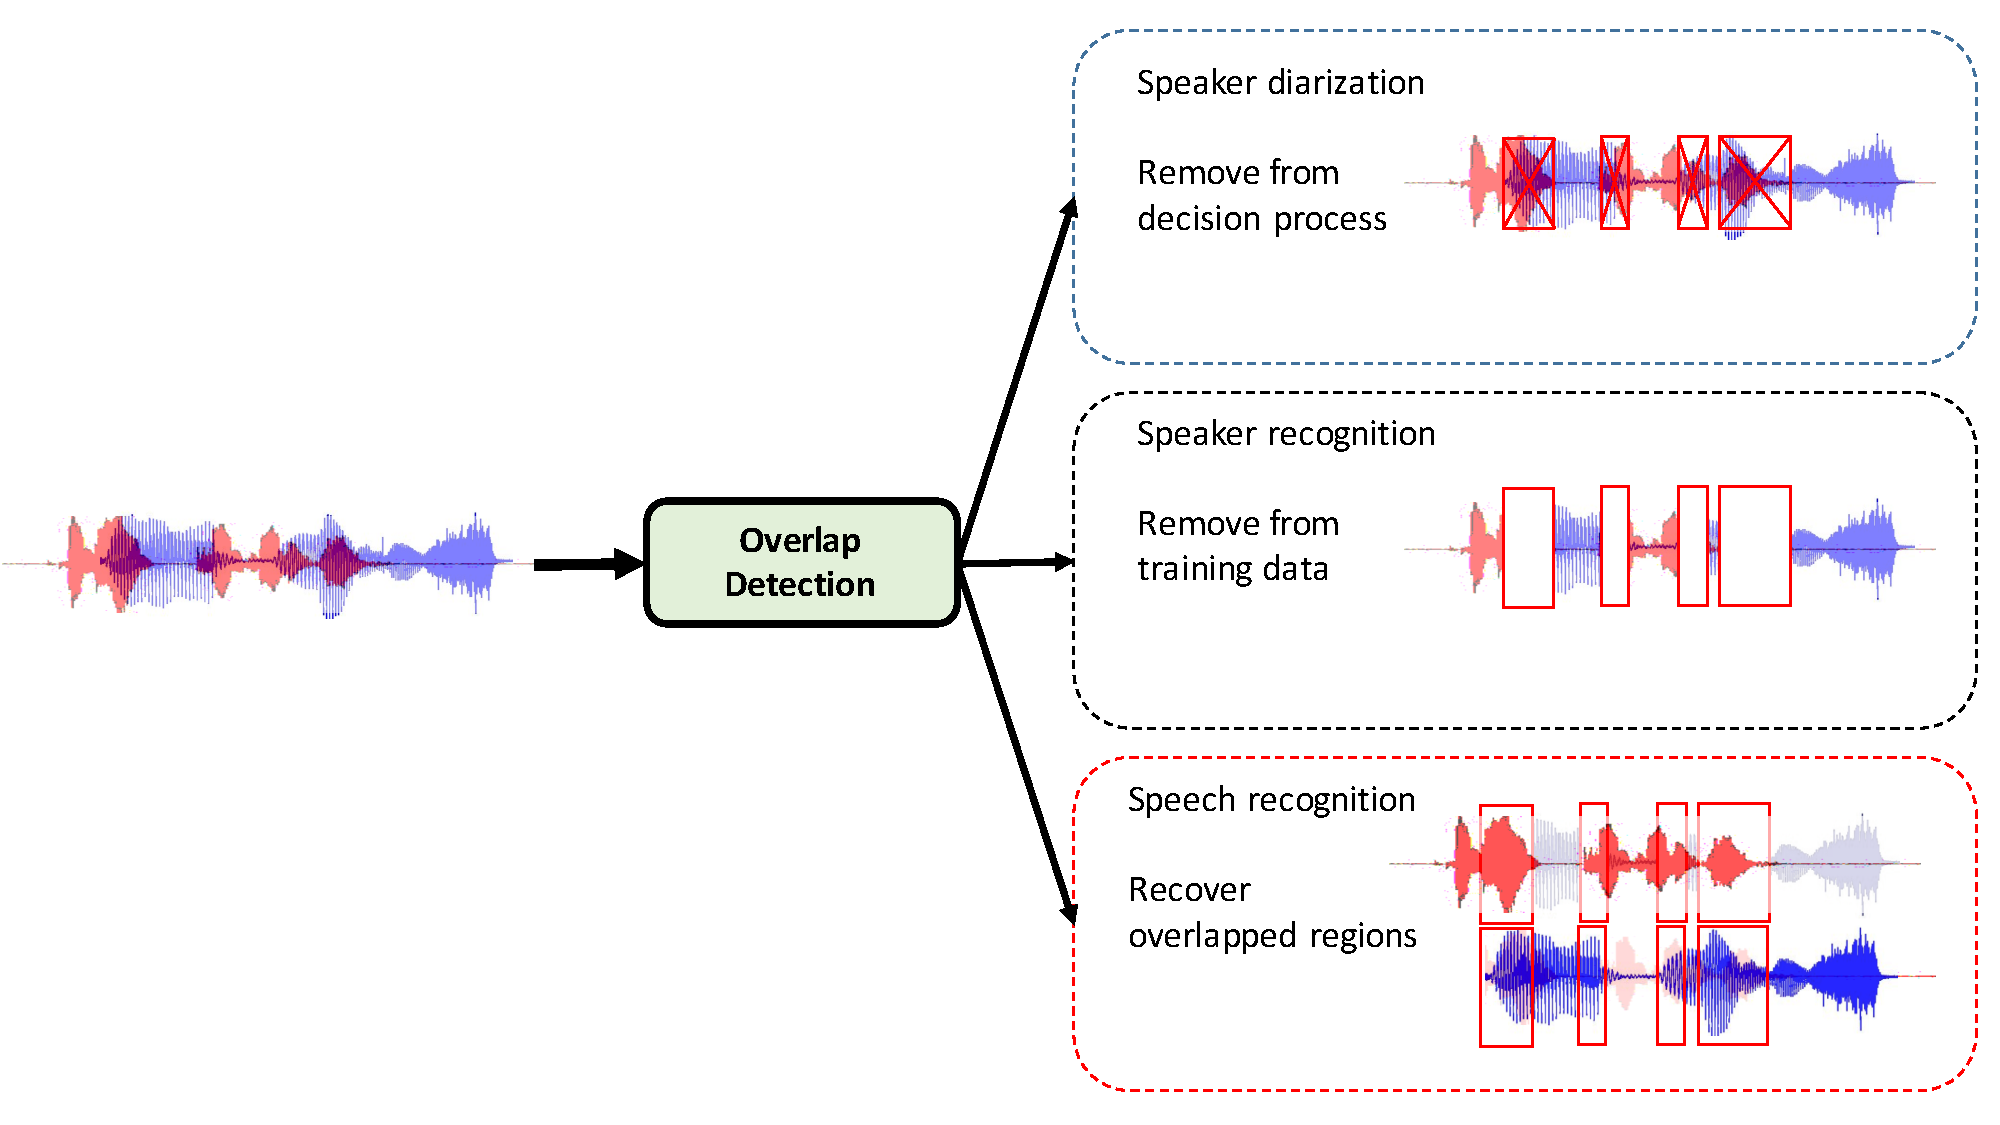
\includegraphics[height = 3in, width=0.9\textwidth]{figures/overlap_detection_applications}
	\vspace{-3mm}
	\caption{\it Applications of overlap detection. Top: In speaker diarization, removing ignoring overlapped regions provides a more fair assessment of diarization performance. Middle: Removing overlaps from in speaker recognition increases the reliability of training data. Bottom: Overlap detection results can be used as an initial step to recover overlapped regions.}
	\label{fig:overlap_applications}
	\vspace{-3mm}
\end{figure}


\newpage
\section{Background}
\label{sec:ch2_methods}

Traditionally, studies have used spectral harmonicity as a key factor in detecting overlapped speech~\cite{nav_icassp13,smolenski_tut}. 
This approach is motivated by the fact that two fundamental frequencies exist in most instances of overlapped speech which disarranges the harmonic structure observed in single-speaker speech. 
As a side-note here, we point out that most of the focus in overlapped speech has been at regions where both speakers produce ``voiced'' speech. In~\cite{morgan_cochannel} a classification of different types of segments in co-channel speech is presented. Figure~\ref{fig:morgan_v_uv_table} is adopted from~\cite{morgan_cochannel}. 

\begin{figure}[h!]
	\centering
	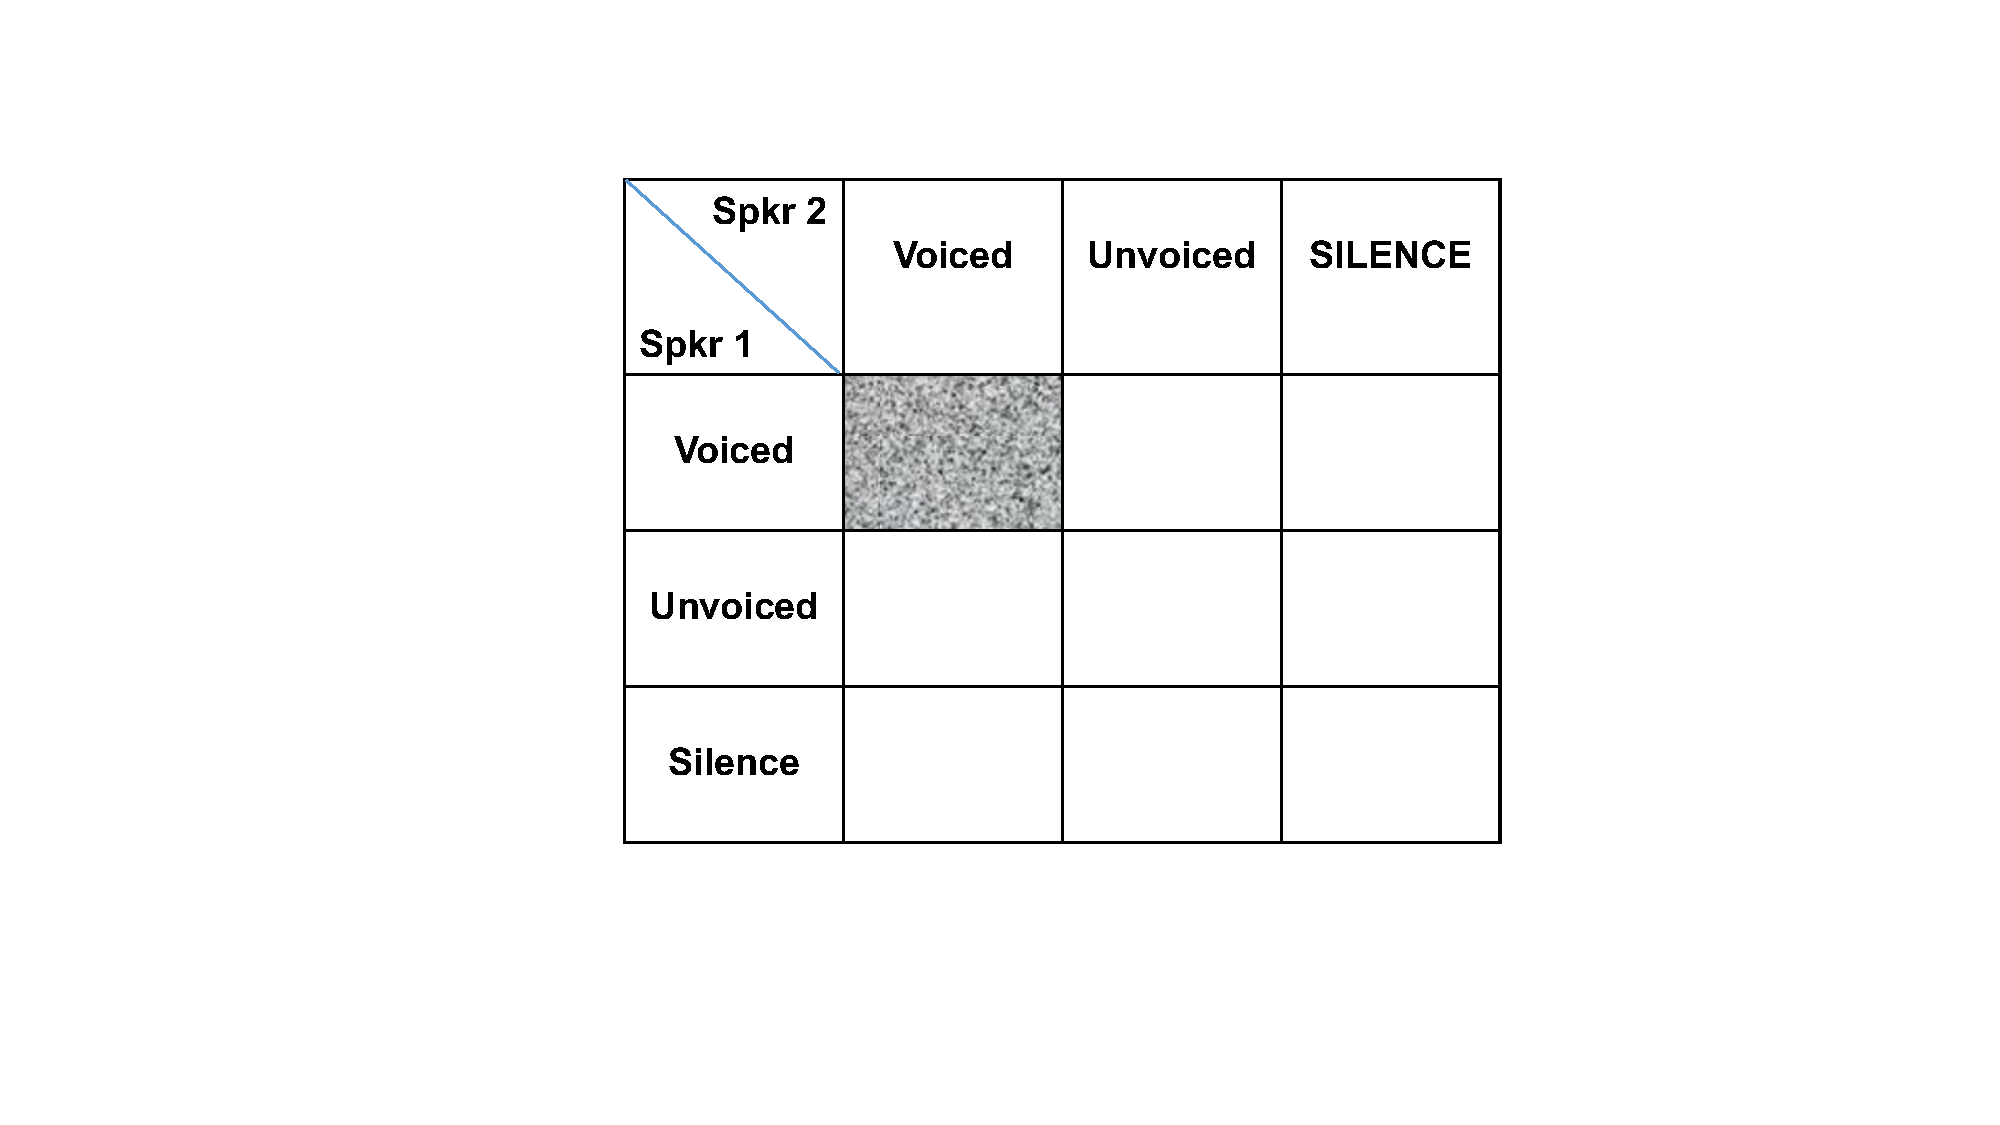
\includegraphics[height = 2.5in, width=0.5\textwidth]{figures/morgan_v_uv_table}
	\caption{\it Classification of different segments in a co-channel file. In overlap detection we are interected in 
		the voiced-voiced (shaded) region.}
	\label{fig:morgan_v_uv_table}
\end{figure}

Most of the attention in this study will also be on the voiced-voiced cell, since detecting other regions is far more difficult and voiced segments are more important for speaker recognition, which is the theme of this thesis. 
A more detailed classification of overlapped regions is presented in~\cite{nav_icassp13}, where a grid containing all phones is used to rank-order overlapped segments in terms of difficulty. 
The analysis in~\cite{nav_icassp13} expands Fig.~\ref{fig:morgan_v_uv_table} as shown in Fig.~\ref{fig:nav_v_uv_table}. 
General consensus is to focus on detecting voiced-voiced overlap detection, which from now on we will refer to as overlap detection. 

\begin{figure}[h!]
	\centering
	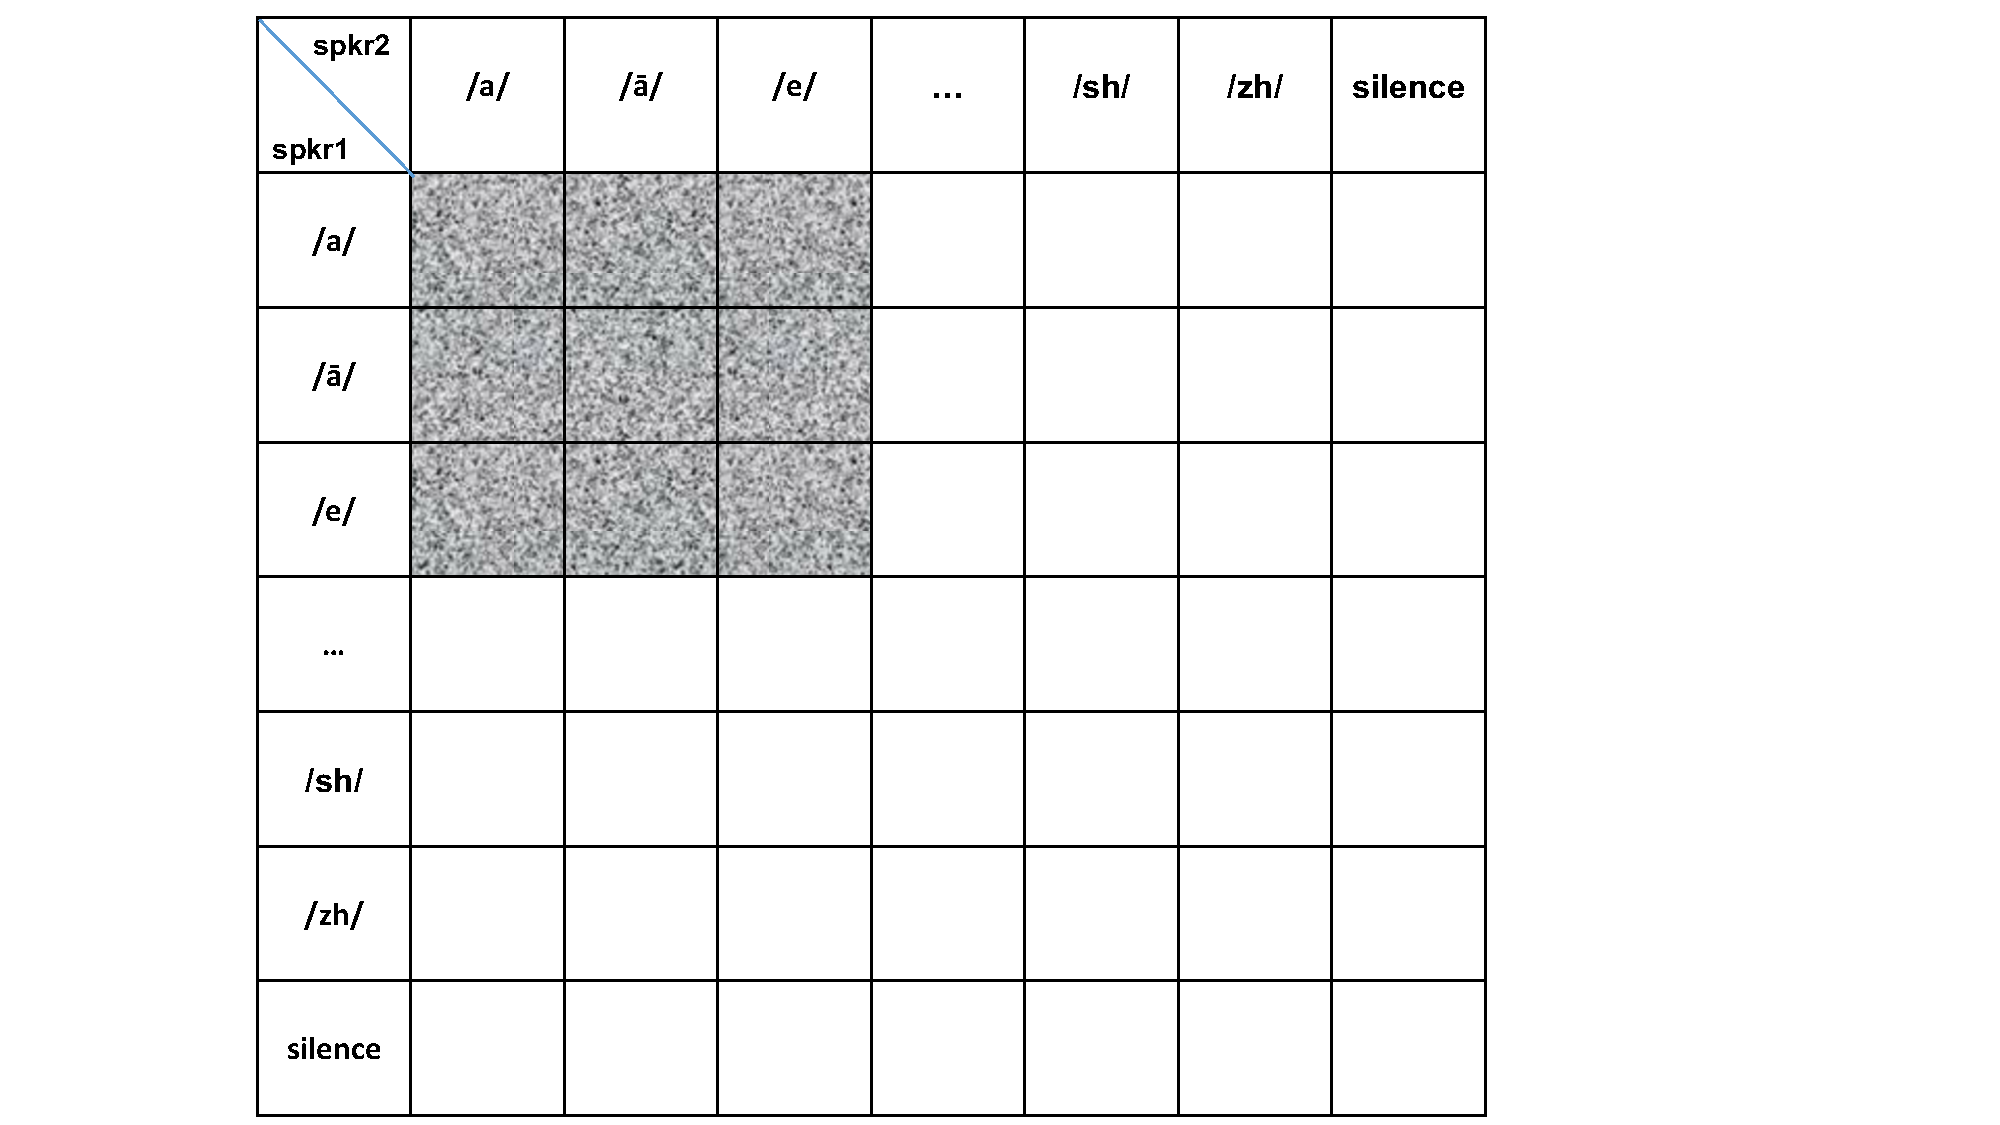
\includegraphics[height = 4in, width=0.7\textwidth]{figures/nav_v_uv_table}	
	\caption{\it phone-based expansion of overlapped segments in Fig.~\ref{fig:morgan_v_uv_table}.}
	\label{fig:nav_v_uv_table}
\end{figure}

Concentrating on voiced speech yields more discriminating harmonic structures. 
Essentially, the defining factor here is that single-speaker voiced spectra are represented as harmonics of a single fundamental frequency. 
The presence of overlapping voiced speech introduces harmonics of a second fundamental frequency, such secondary harmonics are unlikely to be exactly aligned with those of the first speaker. 
In~\cite{sapvr_2000}, the peak-to-valley ratios in frame-based spectral autocorrelations are introduced as a discriminating feature for overlapped speech detection through the same assumption. 
Spectral flatness measure, the ratio of geometric to arithmetic means calculated from spectral bins in a speech frame, has also been used as a measure to capture harmonicity and has been used to detect the presence of overlapped speech~\cite{nav_icassp13}. 
Another related characteristic is observed when monitoring fundamental frequencies along time. 
Adjacent pitch period comparison (APPC) presented in~\cite{appc2001} uses the temporal variation of estimated ``pitch'' periods as a measure to detect ``usable'' speech with the assumption that temporal variations of adjacent pitch periods are significantly higher in overlap. 
A multi-pitch tracking algorithm proposed in~\cite{Dwang_03_trans} was used in~\cite{Dwang_03} to estimate coexisting fundamental frequencies in the presence of multiple speakers. 
Regions where more than one fundamental frequency is estimated are labeled as overlap. 
The multi-pitch tracking technique described in~\cite{Dwang_03_trans}, decomposes speech into sub-bands and pitch estimation is only performed on reliable sub-bands. 

A slightly different, yet fundamentally similar, approach to distinguish overlapped speech is to use speech kurtosis which measures higher order moments of the signal statistics~\cite{Wrigley_05}. 


A number of studies have considered investigating spectral characteristics at formant frequency locations when dealing with overlapped speech. 
Giuliani et al. use a filter-based approach to improve speech recognition rates for different instances of meeting conditions by adding a detection step that separates double-speaker speech from single-speaker audio~\cite{giuliani_meeting}. 
This was accomplished by cascading two-layer sub-band filters to capture formant characteristics. 
Formant frequency information was obtained by filtering the signal at sub-bands with center frequencies and bandwidths corresponding to nominal ${F_1, F_2}$, and ${F_3}$ values for all English vowels. 
One of the reasons Formant-based overlapped speech analysis has received less attention is the difficulties in modeling pole interactions at overlapped regions, which is an issue for linear predictive modeling and other commonly used formant tracking techniques. 
Characterizing pole interactions using standard LP models easily becomes intractable in the presence of more than one source. 
Add to this complication, the unknown speaker locations with respect to each other and the microphone. 
As a result, we focus our attention to nonlinear speech models, some of what have proven more successful in the scenarios described above. 

Nonlinear speech models, including the AM-FM speech model~\cite{maragos_kaiser_quatieri} have been used in previous studies to model speech resonances without any specific requirements for the source signal. 
These energy operators have also been used to deal with signals with more than one source~\cite{maragos_instantaneousenergy}, aka co-channels signals~\footnote{Co-channel is a more general terminology used to described multi-component signals. 
In the case of speech, co-channel speech may refer to any single-channel recording that contains speech from multiple speakers, regardless of whether there is overlap.}. 
Maragos et al. use higher order energy operators to develop an algorithm that simultaneously demodulates the components of a co-channel mixture in AM-FM modulated signals~\cite{maragos_instantaneousenergy}. 
Litvina et al. separate speech from music using the Teager energy operator (TEO) separation algorithm~\cite{maragos_kaiser_quatieri}~\cite{Litvin2010}, where they used the extracted components to design a time-varying filter and suppress the interfering signal. 
Similar multicomponent signal decomposition techniques have been addressed using energy operators to separate narrow-band signals~\cite{Linicassp95,hu12_nullspacepersuit,santhanam_maragos_2000}. 

Our goal is to incorporate sub-band analysis to design a technique suitable for {\bf overlapped speech detection}. 
Two algorithms are proposed that incorporate sub-band analysis for overlap detection: 
\begin{itemize}
	\item using Teager-Kaiser energy operator (TEO) methods on narrow-band components to detect speech harmonics, 
	\item apply cosine functions across sub-band outputs to magnify the presence of multiple harmonics. 
\end{itemize}



\subsection{Baseline features}
\label{ssec:baseline}
Bellow, a collection of overlap detection features are presented that have previously been used to detect overlapped regions~\cite{nav_icassp13,boakye_thesis,sapvr_2000}. 
%We note that all features were implemented based on the information provided in the publications, which are cited in each case. %adapted from other centers based on the information provided in publications. Although we tried to eliminate any chance of bias in the experiments, chances are that the results would have been different had the original authors implemented their methods for these experiments. 
To the best of our knowledge, overlap detection results on the GRID database (see Sect.~\ref{sec:data}) have not been reported for any of the following features, therefore the only reference for comparison are in-house implementations. %The out-of-house features used in this study are:

\begin{itemize}
	\item {\it Speech kurtosis}: Kurtosis has been reported as an effective measure to detect the presence of multiple speakers in overlapped signals by several studies~\cite{Wrigley_05,boakye_thesis,temple_kurtosis}. 
	It has been shown that overlapped speech exhibits lower kurtosis compared to single-speaker speech~\cite{leblanc_deleon98}. The kurtosis of a zero-mean random variable $x$ is defined as:
	
	\begin{equation}
	\label{eq:kurtosis}
	k_x = \frac{E\{x^4\}}{(E\{x^2\})^2}
	\end{equation}
	\vspace{1mm}
	In this case $x$ refers to speech samples in a given frame. 
	\item {\it Spectral flatness measure (SFM)}: The ratio of geometric to arithmetic means of spectral magnitudes across frequency within each frame~\cite{nav_icassp13}. For the $i^{th}$ frame:
	\begin{equation}
	\label{eq:kurtosis}
	sfm_i = \frac{\frac{1}{N}\sum_{n=1}^{N}{X(f_n)}}{^N\sqrt{\prod_{n=1}^{N}{X(f_n)}}}
	\end{equation}
	\vspace{1mm}
	where $X(f_n)$ corresponds to the magnitude spectrum at frequency $f_n$ and {N} is the total number of frequency bins. 
	\item {\it Spectral autocorrelation peak-valley ratio (SAPVR)}: described briefly in Sec.~\ref{sec:intro}, this feature uses the dominance of peaks in the spectral autocorrelation in each frame as a measure to detect overlaps~\cite{sapvr_2000}. 
\end{itemize}

\newpage
\section{Data: Monaural Speech Separation Challenge}
\label{sec:data}
Before moving forward, a description of the data used in the monaural speech separation challenge is provided. 
This data is used throughout the chapter in the analysis of overlapped speech. 
Since the prime focus here is overlapped speech and its physical attributes, we rely on independent cross-talk data for the experiments (see definition in Chapter~\ref{chap:intro}). 

The data used in our controlled experiments is from the monaural speech separation and recognition challenge (aka speech separation challenge (SSC))~\cite{cooke20101}. 
The objective in the SSC was to permit a large-scale comparison of techniques for the overlapped speech problem~\cite{cooke20101}. 
Participants were asked to identify keywords in sentences spoken by a target talker when mixed into a single channel with a background talker speaking sentences of the same structure but with different content. 
The data used in SSC was obtained from the larger GRID corpus~\cite{cooke_JASA_SSCD}, which is a multi-talker audio-visual sentence corpus that supports computational-behavioral studies in speech perception. 
In this study, only the audio content is used. 
The audio consists of 1000 sentences spoken by each of 34 talkers (18 male, 16 female). The sentences are structured in the following format.
\\\\
{\small \bf \textless command\textgreater\textless color\textgreater\textless preposition\textgreater\textless letter\textgreater\textless number\textgreater\textless code\textgreater}
\\\\
For example, ``lay white at X six now''.

Seven overlapped sets are available, one clean and the rest are composed of sentence pairs that are artificially summed at 6 signal-to-interference ratios (SIR) (+6, +3, 0, -3, -6, -9 dB). 
Since file durations are short (typically less than 5 seconds) and the utterances contain negligible pauses, it is reasonable to consider the average SIR values, provided for each file, a fair representation of the amount of overlap. 
It is also safe to assume that a given file is all speech, removing the need to run speech activity detection to separate speech from silence. 
This assumption justifies labeling a ``clean'' file (no overlap) as single-speaker. 
Alternatively, it is also reasonable to consider an entire overlapped signal double-speaker (aka overlap) (see Fig.~\ref{fig:overlap_example}). 
All files have been down-sampled to 8kHz to match telephone recordings. 
Note that the experiments conducted in this study do not comply with the objectives of the speech separation challenge described in~\cite{SSC_link}. 

% Figure added because of Reviewer3 and 1's comment:
\vspace{0mm}
\begin{figure}[h!]
	\centering
	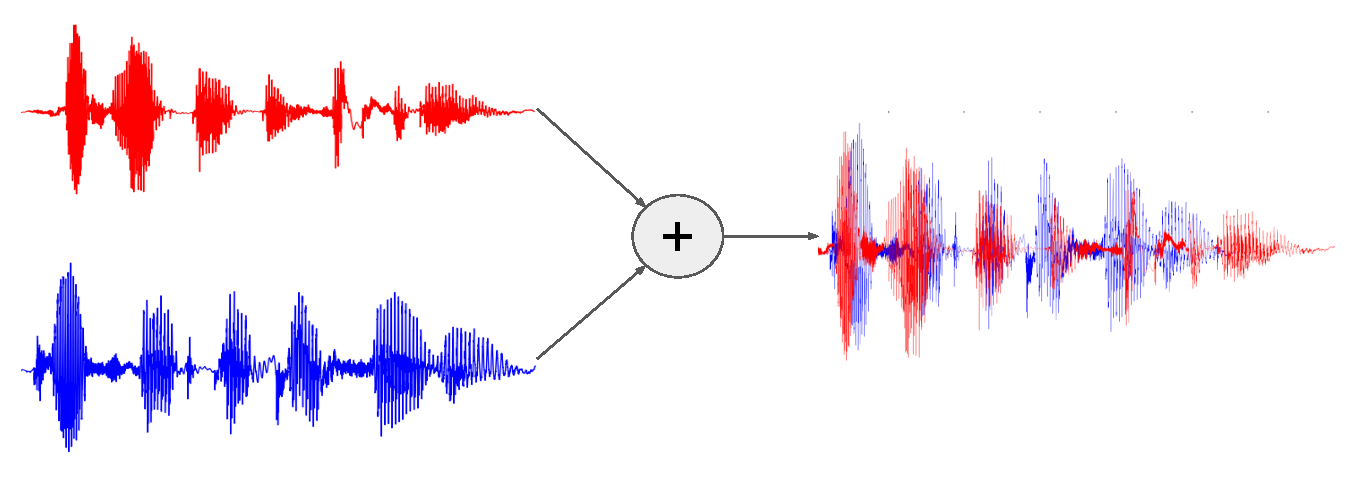
\includegraphics[height =1.8in, width=0.7\textwidth]{figures/GRID_example_overlap-crop}
	\vspace{-2mm}
	\caption{\it 
		Example of the mixing process for a 0dB SIR overlapped signal. As shown on the right, it is fair to assume that overlap occurs throughout the signal.}
	\label{fig:overlap_example}
\end{figure}

% Reviewer1's comment:
The choice of dataset for this study is pertinent to the investigative objective of this chapter, overlap detection. 
Other studies have also focused on controlled datasets such as TIMIT~\cite{nav_icassp13} as well as realistic datasets including Prof-life-log~\cite{ziaei2013prof,nav_icassp15}, Switchboard~\cite{shokouhi2015}, and UT-Drive in-vehicle conversations~\cite{sathyanarayana2013belt}. 
Some of these studies are described in following chapters. 
Unfortunately, none of the aforementioned datasets are designed to contain significant amounts of overlap. 
One may argue that overlaps exist in conversational speech corpora such as Switchboard or the AMI meeting corpus~\cite{amicorpus}. 
Although it is true that these corpora contain overlapped segments, the amounts of overlap in ``regular'' (aka non-competitive conversations~\cite{schegloff2000overlapping}) is not sufficient for the requirements of this study. 
The reason control is required over the amount of overlap in experiments is to specifically investigate the power of proposed overlap detection systems and not worry about target/non-target imbalances observed in conversational speech. 
Furthermore, the GRID corpus is isolated from variabilities other than overlapped speech, which makes it useful to study the effects of overlap. 
To the best of my knowledge, this dataset is the most organized publicly available corpus that contains large and controlled amounts of overlapped speech (note that we are mostly interested in {\it overlapped speech} and not {\it co-channel speech} as defined and distinguished in the introduction). 
Another advantage of the corpus is the fact that segments are short which makes the definition of a signal-to-interference ratio more appropriate. Had the signals been longer, say a few minutes long, the notion of a signal-to-interference ratio across the entire signal would have been less applicable, due to the non-stationary nature of speech. 

Table~\ref{tab:data_summary} shows some features of the dataset used in this study, including: number of speakers (male and female), average file duration, and overlap conditions. 

\begin{table}[h!]
	\begin{center}
		\begin{tabular}{| c | c |}
			\hline
			\hline
			number of speakers	& 18 (male)  \\
			\hspace{4mm}			&  16 (female) \\
			\hline
			average file duration	&   1.9 (sec) \\ 
			\hline
			noise				& interfering speakers \\
			\hspace{4mm}			& clean,$+6$, $+3$, $0$, $-3$, $-6$, $-9$ dB \\
			\hline
			sampling rate			& $8$ KHz \\
			\hline
			\hline	
		\end{tabular}
		\caption{\it Summary of data used for speaker recognition experiments}
		\label{tab:data_summary}
	\end{center}
\end{table}

\newpage
\section{Pyknogram-based overlap detection}
\label{sec:ch2_Pykno}
The first proposed overlap detection method is a novel approach for overlapped speech detection based on an enhanced spectrogram. 
These spectrograms, called Pyknograms, were first introduced by Potamianos and Maragos in~\cite{potamianos_maragos_icassp95,potamianos_maragos_jasa96} and are calculated by applying multi-band demodulation in the AM-FM speech model framework~\cite{maragos_kaiser_quatieri}{\footnote{The authors in~\cite{potamianos_maragos_jasa96} used the term ``Pyknogram'' which stems from the Greek word ``pykno'' meaning dense. Pyknograms represent highly resonating regions in time-frequency plots as populated scatter plots, hence the term density.}. 
Pyknograms provide a more prominent representation of harmonic trajectories, which are proposed here to be used as a means to detect the presence of interfering speech.

Pyknogram extraction can be considered a 2 step process of obtaining a binary mask of time-frequency units for the amplitude spectrogram. 
\begin{enumerate}
	\item Frequency estimation: Computes resonant frequencies in time-frequency units. The procedure in this step includes: 
	\begin{itemize}
		\item apply a gammatone fiterbank to the speech signal
		\item estimate instantaneous amplitude and frequencies using TEO
		\item block the per sub-band outputs into time frames
	\end{itemize}
	\item Frequency selection: Prunes the estimated frequencies to find the most reliable units.
\end{enumerate}

\subsection{Pyknogram Extraction - Frequency estimation}
\label{ssec:pykno_estimate}
In Pyknograms~\cite{potamianos_maragos_jasa96}, the harmonic structure of speech is enhanced by decomposing spectral sub-bands into amplitude and frequency components. 
This sub-band analysis uses the AM-FM speech model~\cite{maragos_kaiser_quatieri} to decompose speech sub-bands and thereby calculate corresponding instantaneous frequencies and bandwidths. 
To extract Pyknograms, the speech signal is initially passed through a filter-bank (the algorithm has been modified in this study to use logarithmically spaced Gamma-tone filters, while~\cite{potamianos_maragos_jasa96} uses linearly-spaced Gabor filters). 
Filter-bank outputs ($x_i(n)$, in which $i$ represents filter indexes) are then decomposed into amplitude and frequency components using the discrete energy separation algorithm (DESA-1)~\cite{maragos_kaiser_quatieri}, where the per sample frequency of $x_i(n)$ is $f_i(n)$ and the amplitude is $a_i(n)$. Frequency and amplitude estimates for the $i^{th} $sub-band, $x_i(n)$, are:

\begin{equation}
	\label{eq:instfreq}
	f_i(n) = \frac{1}{2\pi}\arccos \Big (1-\frac{\Psi[x_i(n)-x_i(n-1)]}{2\Psi[x_i(n)]}\Big),
\end{equation}
	
	
\begin{equation}
	\label{eq:instamp}
	|a_i(n)| = \sqrt{\frac{\Psi[x_i(n)]}{\sin^2(2\pi f_i(n))}} , \hspace{10mm}i=1,2,...,N_s
\end{equation}
where $n$ is the time sample. $N_s$ is the number of sub-bands in the filter-bank and $\Psi(.)$ is the discrete energy operator, defined for any given signal, $x(n)$, as:
\begin{equation}
	\Psi [x(n)] = x^2(n)-x(n-1)x(n+1).
\end{equation}


\begin{figure}[h!]
	\centering
	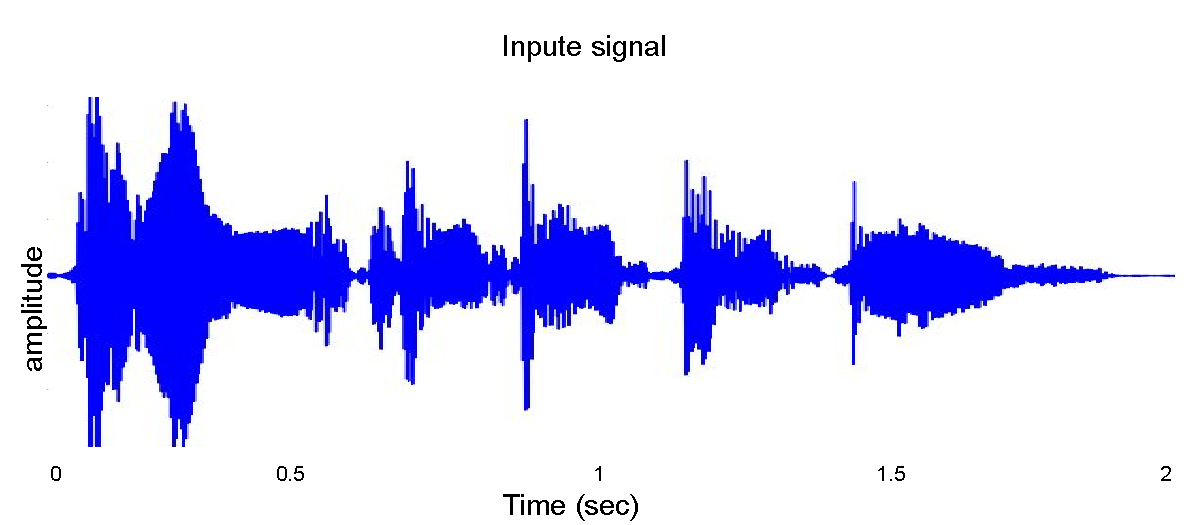
\includegraphics[height=2in, width=1\textwidth]{figures/teo_signal}
	\caption{\it Input signal.}
\end{figure}
	
\vspace{1.0mm}
\begin{figure}[h!]
	\centering
	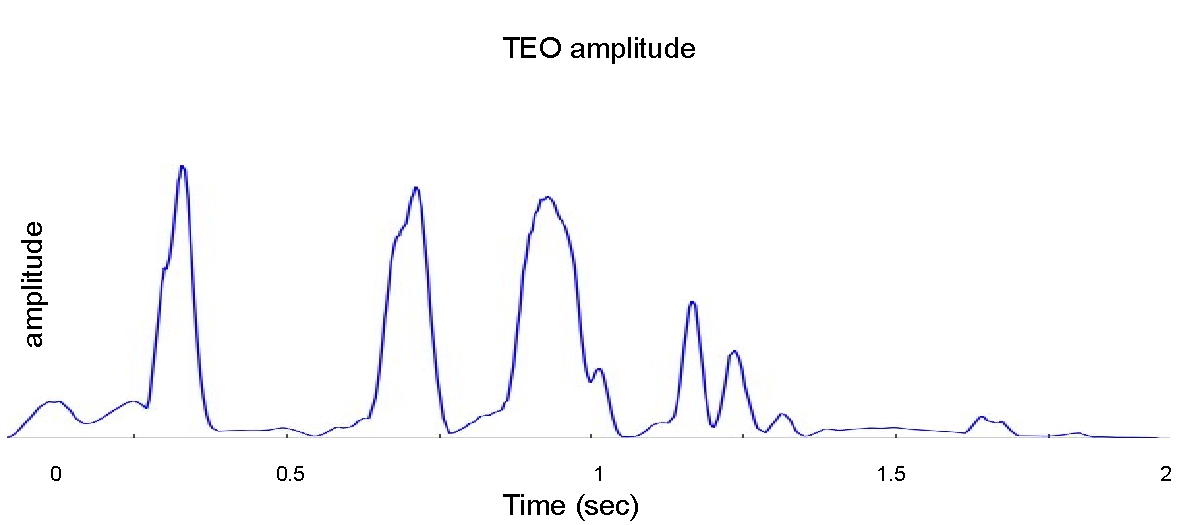
\includegraphics[height=2in, width=1\textwidth]{figures/teo_amp}
	\caption{\it Outputs of DESA-1: Signal amplitude component estimated using TEO, Eq.~(\ref{eq:instamp}).}
\end{figure}

\begin{figure}[h!]
	\centering
	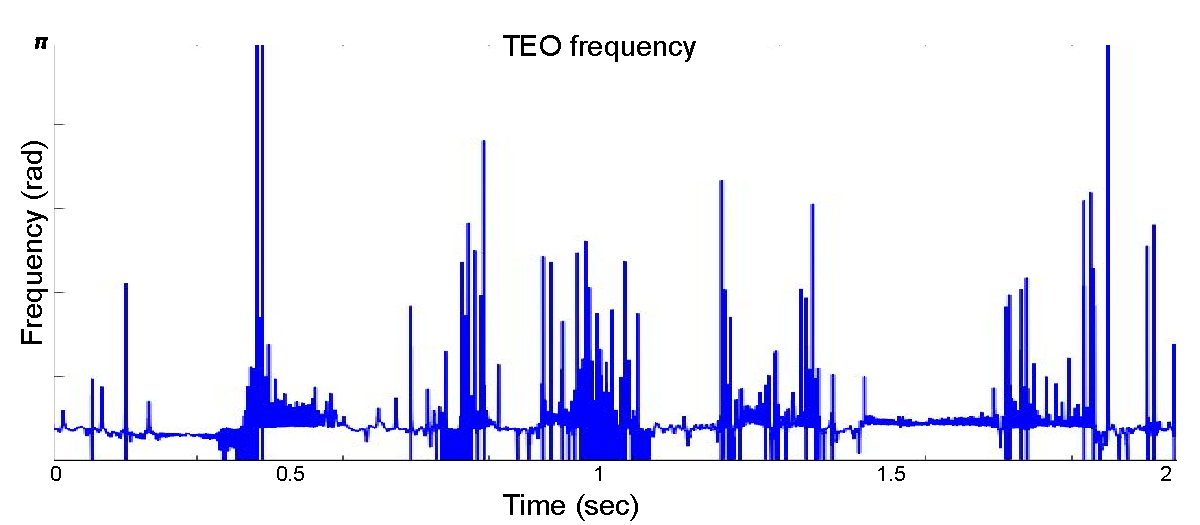
\includegraphics[height=2in, width=1\textwidth]{figures/teo_freq}
	\caption{\it Outputs of DESA-1: Signal frequency component estimated using TEO,  Eq.~(\ref{eq:instfreq}).}
\end{figure}

A weighted average of the instantaneous frequencies, $F_w$, is estimated over $25msec$ windows (aka frames), indexed by $t$. 
Together sub-band analysis and time framing results in time-frequency units $(t,i)$, where $i$ corresponds to the frequency sub-band index and $t$ corresponds to frames~\cite{cohenlee90}.
Instantaneous frequencies are weighted using the estimated signal power ($|a_i(n)|^2$). 
The average frequency computed for each time-frequency unit can be viewed as the $1^{st}$-order moment of instantaneous frequencies.  


\begin{equation}
\label{eq:weighted_f}
F_w(t,i) = \frac{\sum_{n_t}^{n_t+T - 1}f_i(n)a_i^2(n)}{\sum_{n_t}^{n_t+T - 1}a_i^2(n)},
\end{equation}
$T$ is the number of samples per frame, from $n = n_t$ to $n = n_t+T - 1$, in which $n_t$ is the beginning sample of frame $t$. 
The algorithm also provides a way to estimate weighted bandwidths for the frequency component, (\ref{eq:weighted_bw}). 
What are referred to here as bandwidths are essentially $2^{nd}$-order frequency moments. 

\begin{equation}
\label{eq:weighted_bw}
B_w(t,i) = \sqrt{\frac{\sum_{n_t}^{n_t+T-1}(\overset{\boldsymbol .}{a_i}(n) /2\pi)^2+(f_i(n)-F_w(t,i))^2a_i^2(n)}{\sum_{n_t}^{n_t+T-1}a_i^2(n)}},
\end{equation}
where $f_i(n)$ and $a_i(n)$ are instantaneous frequency and amplitude values from (\ref{eq:instfreq}) and (\ref{eq:instamp}). 
In (\ref{eq:weighted_f}), the instantaneous frequencies are averaged over the $t^{th}$ frame using squared instantaneous amplitudes as weights. 
$\overset{\boldsymbol .}{a}(n)$ is the first difference of $a(n)$ (i.e., $a(n) - a(n-1)$). 
The per-frame values of $F_w$ provide initial estimates of spectrogram peaks. 
This results in a time-frequency, {$t$-$f$}, representation of the overall signal. 


In~\cite{potamianos_maragos_jasa96}, the bandwidths, $B_w$, defined in (\ref{eq:weighted_bw}) are used for analysis purposes. 
Here, they are used in overlap detection systems to determine the reliability of $t-f$ units. 
The assumption is that large Pyknogram bandwidths correspond to higher uncertainty in frequency estimates. 
This assumption is investigated in following sections by adding an uncertainty term to frequency estimates proportional to the estimated bandwidth:

\begin{equation}
\label{eq:jitter_f}
\tilde F_w(t,i) = F_w(t,i) + \epsilon_t,
\end{equation}
where
\begin{equation}
\label{eq:jitter_pdf}
\epsilon^i_t \sim\ \mathcal{N}(0,B_w(t,i)).
\end{equation}

\subsection{Pyknogram Extraction - Frequency selection}
\label{sssec:pykno_select}
In the second step of Pyknogram extraction, dominant harmonic peaks are selected by comparing the average frequency estimates with filter-bank center frequencies. 
According to~\cite{potamianos_maragos_jasa96}, points at which filter-bank center frequencies coincide with the weighted frequency estimates from (\ref{eq:weighted_f}) are more reliable in estimating spectrogram peaks. 
In Sect.~\ref{ssec:pykno_estimate}, it was shown how resonant frequencies are estimated using Teager energy operators. 
A considerable number of these frequencies can be omitted from the list of candidate frequencies. 
The assumption being that frequency estimates are more accurate when resonances align with a filter in the filter-bank. 
This defines the condition through which initial $F_w$ values are tested to detect whether they correspond to prominent peaks. At frame $t$: 
\vspace{0mm}
\begin{equation}
\label{eq:RF1}
F_w(t,i) = F_c(i)  \quad \iff \quad \{i \in peaks\}
\vspace{1mm}
\end{equation}
where $F_c(i)$ is the center frequency of the $i^{th}$ filter in the gammatone filter-bank. 
Note that center frequencies are distributed in a logarithmic scale. 
Another peak selection condition (as shown in Fig.~\ref{fig:pykno_blockdiag}) is to limit the relative variance of selected frequencies with respect to center frequencies. 

\begin{equation}
\label{eq:RF2}
\Big|\frac{\partial F_w(t,i)}{\partial i} \Big| \approx \Big|\frac{F_w(t,i+1) - F_w(t,i)}{(i+1) - i}\Big| < thr, 
\vspace{1mm}
\end{equation}
This condition limits non-harmonic anomalies that break the patterns in regular speech harmonics. 
Since such patterns are frequently observed in overlapped data, this restriction can be removed from the peak-picking step.  

\begin{figure}[h!]
	\centering
	\vspace{0mm}
	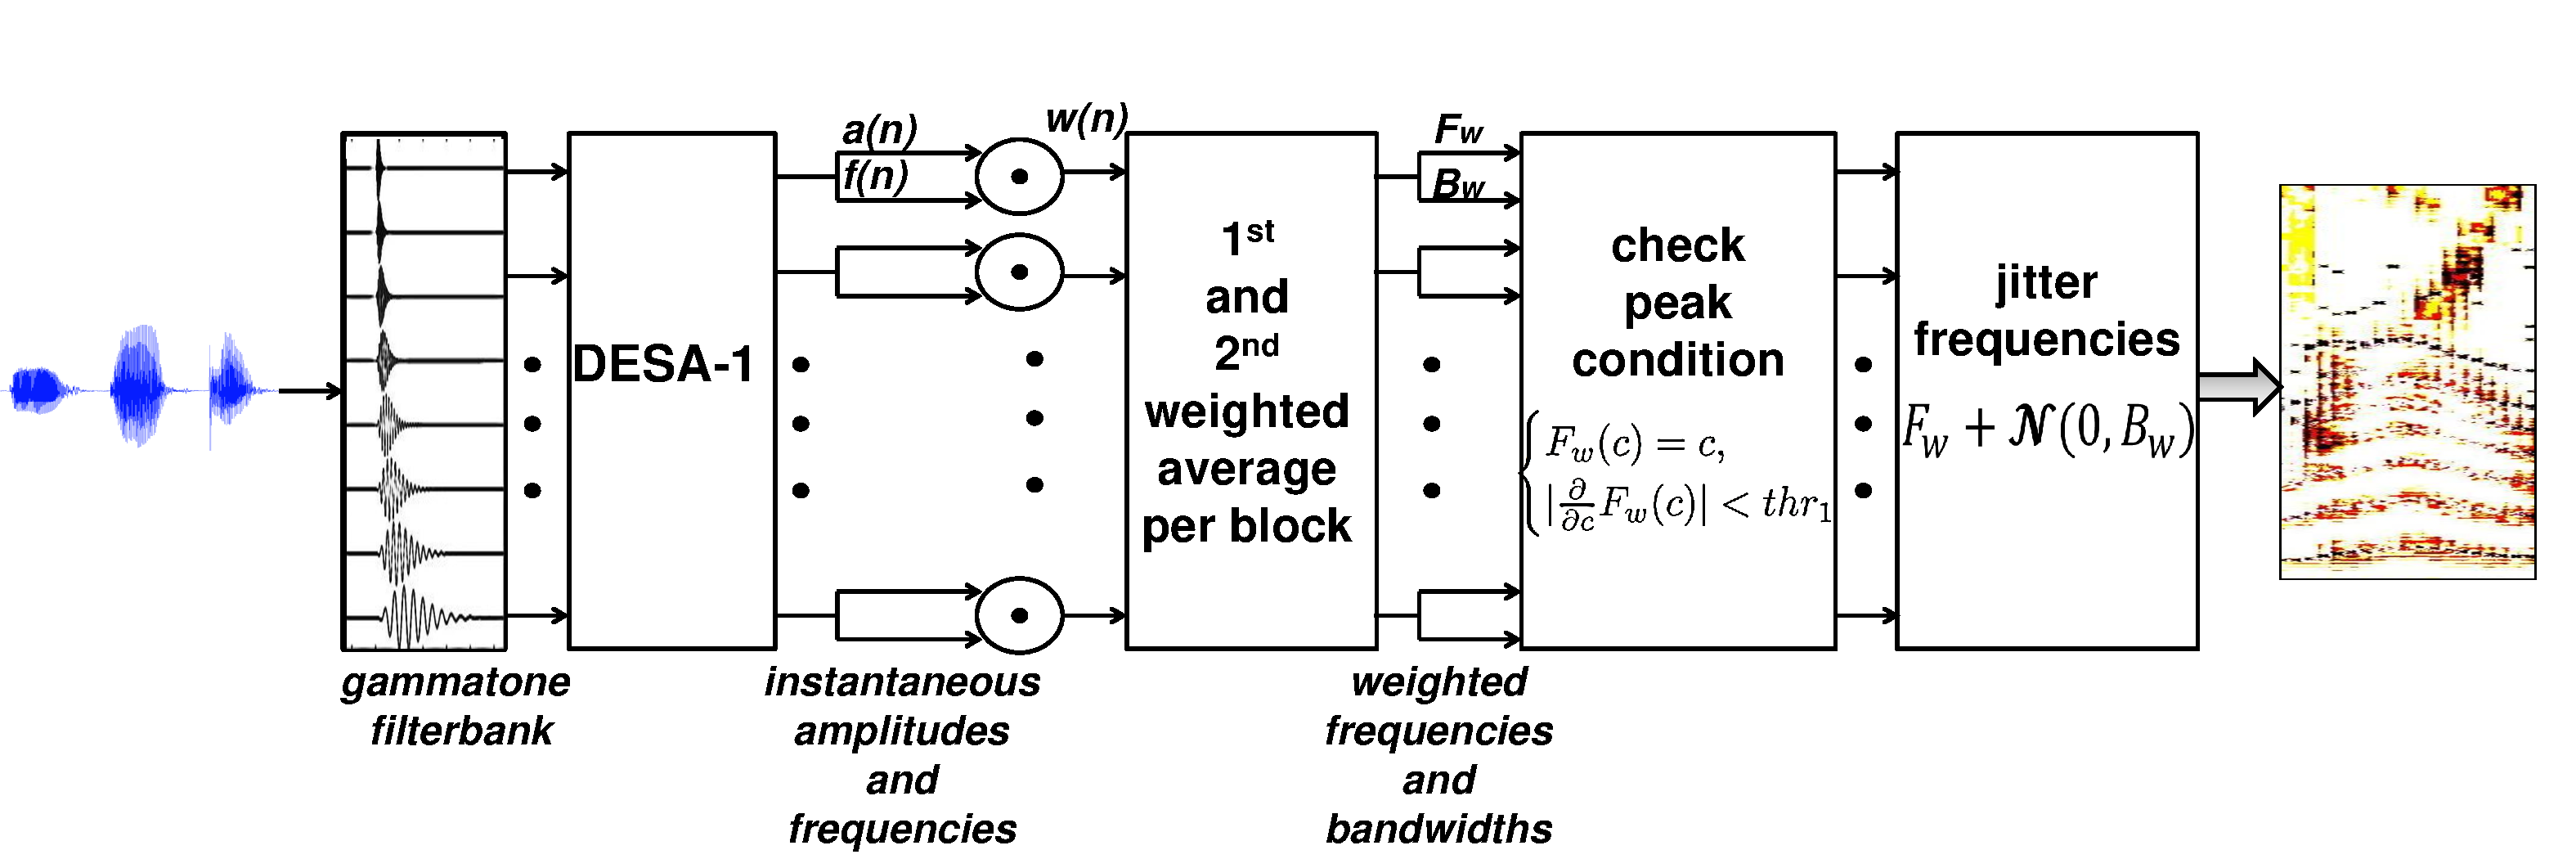
\includegraphics[height = 2.5in, width=1\textwidth]{figures/pyknogram_blockdiagram}
	\vspace{-3mm}
	\caption{\it Pyknogram extraction block-diagram.}
	\label{fig:pykno_blockdiag}
	\vspace{-3mm}
\end{figure}


One of the advantages of the peak-picking constraint in (\ref{eq:RF1}) is the quantization of spectrograms onto filter-bank center frequencies. 
This allows the mapping of all signals onto a unified space defined by the filter-bank, which enables reliable comparison within the time-frequency space. 

Using an energy operator based approach helps avoid assumptions on the number of speakers in the signal. 
AM-FM decomposition is suitable since it relies on signal resonances and does not restrict signals to a specific structure or number of speakers (as opposed to models such as linear prediction). 
The final time-frequency representation is called a Pyknogram, $S_{pyk}(t,i)$, which is a function of time ($t$) and frequency index ($i$). 
$S_{pyk}(t,i)$ is obtained by applying a binary mask to the gammatone time-frequency amplitudes estimated, $A(t,i)$, from (\ref{eq:instamp}) in the following manner:
\begin{equation}
\label{eq:amplitude_spectrum}
A(t,i) = \frac{1}{T}\sum_{n_t}^{n_t+T - 1}a_i^2(n),
\end{equation}
The binary mask that results in $S_{pyk}(t,i)$ uses only amplitude values that are selected from (8) and (9). 


\begin{equation}
S_{pyk}(t,i)=\begin{cases}
A(t,i), & \text{if $F_w(t,i)$ satisifies (\ref{eq:RF1})and(\ref{eq:RF2})}.\\
0, & \text{otherwise}.
\end{cases}
\end{equation}
Figure~\ref{fig:pyknograms} shows the binary mask and underlying gammatone amplitude estimates for a given speech sample. 

\begin{figure}[h!]
	\centering
	\vspace{4mm}
	\textbf{Pyknogram}\par\medskip
	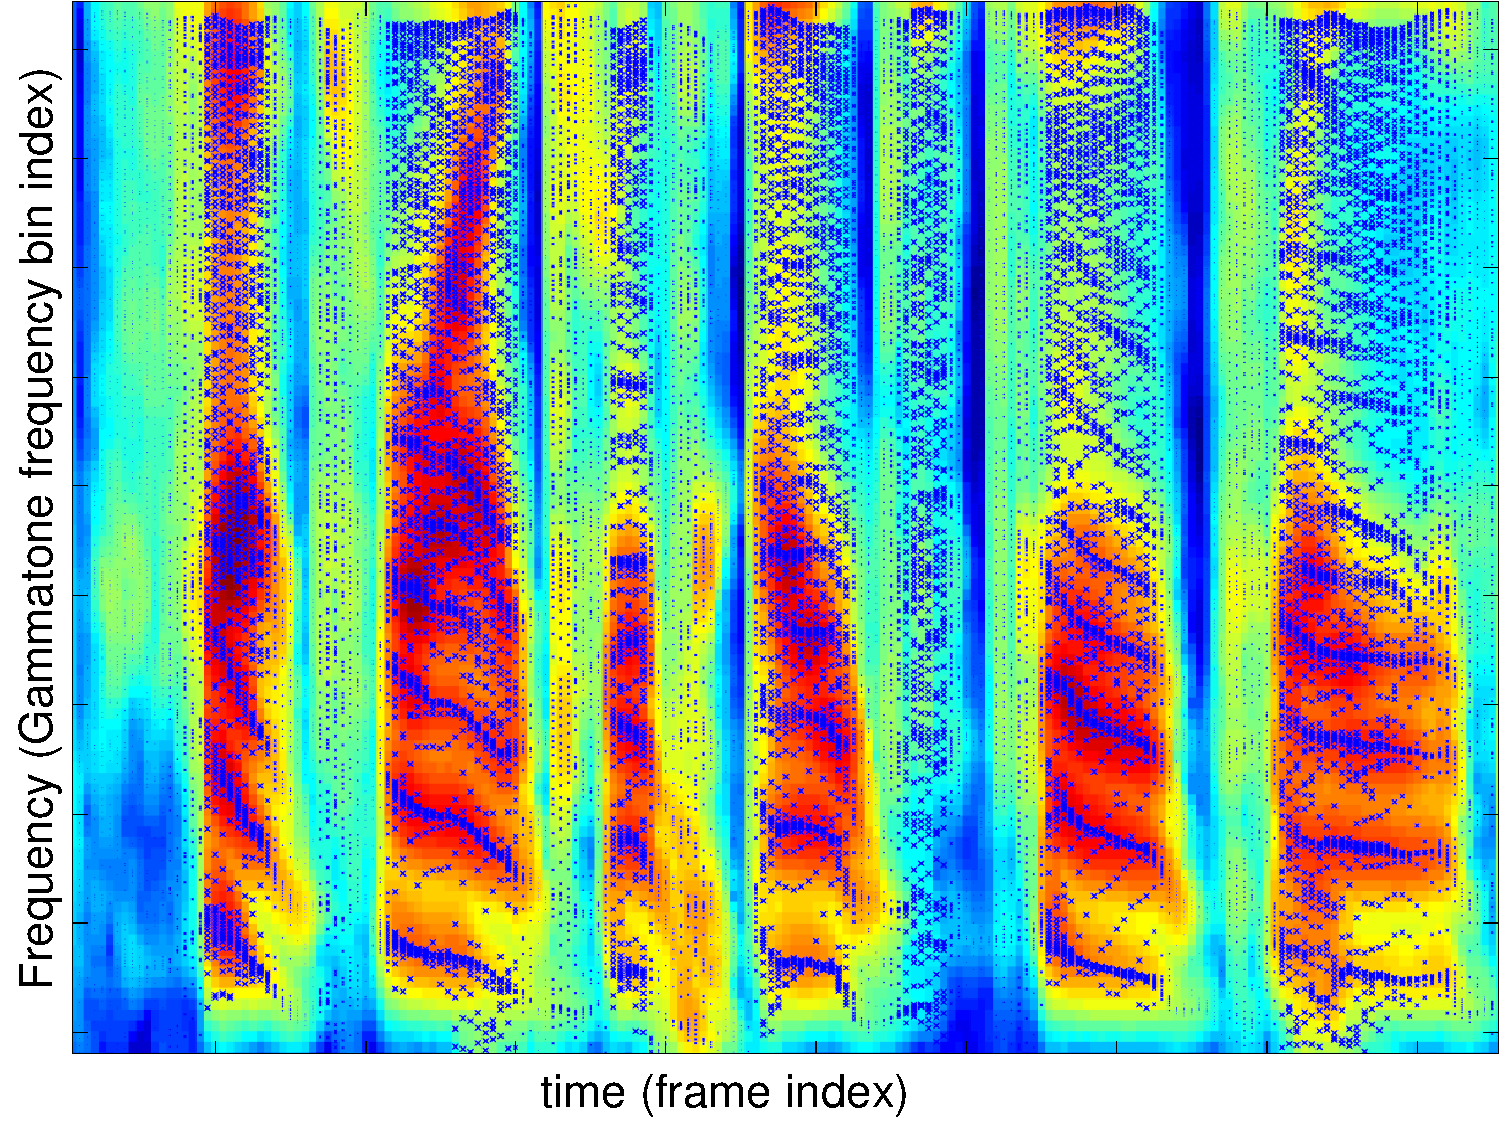
\includegraphics[height =2.in, width=0.5\textwidth]{figures/pyknogram_vs_spectrogram}
	\vspace{-1mm}
	\caption{\it Pyknogram for a given speech signal. The spectrogram is plotted in the background for comparison. Pyknogram markers have been scaled by the amplitudes of corresponding $t$-$f$ units. Frequencies are scaled to equivalent rectangular bandwidth (ERB) rate.}
	\vspace{-1mm}
	\label{fig:pyknograms}
\end{figure}

The next step is to investigate overlap detection methods using Pyknograms.
Discontinuities in the Pyknogram layout is an indication of interfering speech. 
An analogy for speech harmonic patterns are skiing tracks left behind on a snowy surface. 
In the single-speaker case, the patterns leave parallel tracks that progress relatively slowly over time and correspond to fundamental frequency harmonic tracks. 
In the presence of an interfering speaker, these patterns are distorted by similar but intersecting tracks, which adds sudden jumps along the time axis (as shown in Fig.~\ref{fig:pyknograms_for_overlaps} describing Pyknogram extraction). 
Since speakers are only capable of producing one fundamental frequency at each time instance, it is expected that the harmonic tracks should be consistent across time. 
This keeps harmonics parallel over short time intervals.   
The presence of a second speaker creates harmonic tracks that in general do not follow the same patterns, hence discontinuities are observed along time in Pyknograms. Therefore, Pyknogram variations across adjacent frames can be used to measure overlapped speech.

\begin{figure}[h!]
	\centering
	\vspace{1mm}
	\textbf{Pyknogram close-up}\par\medskip
	\vspace{-1mm}
	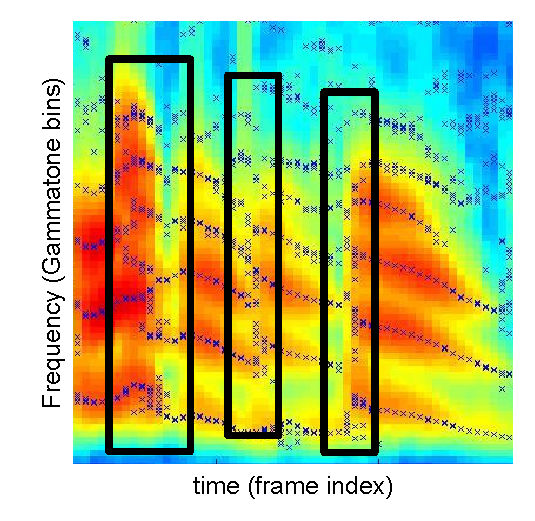
\includegraphics[height =2.0in, width=0.4\textwidth]{figures/co-channel_pyknogram-crop}
	\vspace{-1mm}
	\caption{\it A closer look on Pyknograms for overlapped speech. The enclosed patches show discontinuities that occur in the presence of an interfering speaker.}
	\vspace{-1mm}
	\label{fig:pyknograms_for_overlaps}
\end{figure}

Figure~\ref{fig:pyknograms_for_overlaps} close-up of the Pyknogram for overlapped speech. 
The sudden jumps in Pyknogram frequency locations (shown in blocks) are an indication of two speakers. 

\newpage
\subsection{Unsupervised overlap detection using Pyknograms}
\label{ssec:unsupervised_ovl_det_pykno}
The average Euclidean distance between consecutive frames across all frequencies can be used to detect sudden jumps in Pyknograms along time. 
Much like the technique used for spectral flux estimation~\cite{Rossignol_spectralflux}. 
The distance function, $D_{ovl}$, at frame $t$ is computed as the $2$-$norm$ distance between consecutive Pyknogram frames, $S_{pyk}(t,i)$ and $S_{pyk}(t-1,i)$. 

\begin{equation}
\label{eq:ovl_det_score}
D_{ovl}(t) = \sqrt{\sum_i\Big(\big(S_{pyk}(t,i)-S_{pyk}(t-1,i)\big)^2\Big)}
\end{equation}
which results in a frame-based value for overlap distances. 
Future sections will investigate using longer time windows by averaging $D_{ovl}$ of adjacent frames. 

Overlapped segments are expected to have higher $D_{ovl}$ values as compared to single-speaker speech. 
Figure~\ref{fig:pyknograms_for_overlaps} shows instances where sudden jumps are observed in the pyknogram of an overlapped signal. 
The average value of these distances for all frames in a speech segment corresponds to the amount of overlapped regions (higher values are associated with greater overlap). 

The performance of the proposed detection metric is evaluate on overlapped speech on the GRID database~\cite{SSC_link} (see Sect.~\ref{sec:data} for more details on GRID). 
A key factor that determines the difficulty of detecting the presence of overlapped speech is the signal-to-interference (SIR) value. 
SIR is formally defined as the average energy of the foreground speaker to the energy of the background speaker, in dB. 
Of course, in the case of overlap detection, one speaker is not favored as the foreground over the other. 
Therefore absolute SIR values should be used for overlap detection. 
Greater absolute SIR corresponds to regions where one of the speakers has lower impact on the signal energy. 
It is therefore more difficult to detect the occurrence of overlap in signals as the absolute SIR increases from zero.  
From here on after, when we use SIR, we imply its absolute value. 

Another important factor in detecting overlap is that the SIR value will change across different frames within a single file, which is due to the non-stationary nature of speech. 
This poses major restrictions on the effectiveness of overlap detection evaluation, since providing frame-based ground-truth becomes unrealistically difficult. 
One must therefore rely on ensemble measurements over complete speech files for which the average SIR is known. 
We therefore introduce the segment-based $D_{ovl}$ value which is the ensemble average of all frames within $M$ second intervals. 
\begin{equation}
\label{eq:seg_dovl}
^{M}D_{ovl}(t) = \sum_{t = t}^{t+\lfloor \frac{M}{T_s} \rfloor} D_{ovl}(t)
\end{equation}
where $T_s$ is the length of frame shift (in seconds), used here to determine the number of frames in an $M$ second interval. 
This notion is illustrated in Fig.~\ref{fig:compare_perframe_and_perfile_ovldethist}, where $D_{ovl}$ distributions (histograms) extracted on a per-frame basis are compared with ensemble $D_{ovl}$ distributions associated with longer durations ($2$ seconds). 
$D_{ovl}$ for $2$ second samples is calculated by averaging per-frame values. 
The ``scores'' ($D_{ovl}$ values) in Fig.~\ref{fig:compare_perframe_and_perfile_ovldethist} are pyknogram distances calculated using (\ref{eq:ovl_det_score}). 
The top figure (Fig.~\ref{fig:compare_perframe_and_perfile_ovldethist}-a), shows the distribution of scores per {\it frame} (i.e. $25$msec intervals) for overlapped (target) and clean (non-target/single-speaker) data.  
Figure~\ref{fig:compare_perframe_and_perfile_ovldethist}-b shows the ensemble score distributions (average score over all frames in $2$ second segments). 
The task in overlap detection is to separate the two classes in each plot (dark blue from light blue). 
As observed in these distributions, the per-frame classes are almost indistinguishable (Fig.~\ref{fig:compare_perframe_and_perfile_ovldethist}-a), while in Fig.~\ref{fig:compare_perframe_and_perfile_ovldethist}-b the classes show much better separation. 


\begin{figure}[h!]
	\centering
	\vspace{0mm}
	\textbf{Ensemble vs. frame-based decisioning}\par\medskip	
	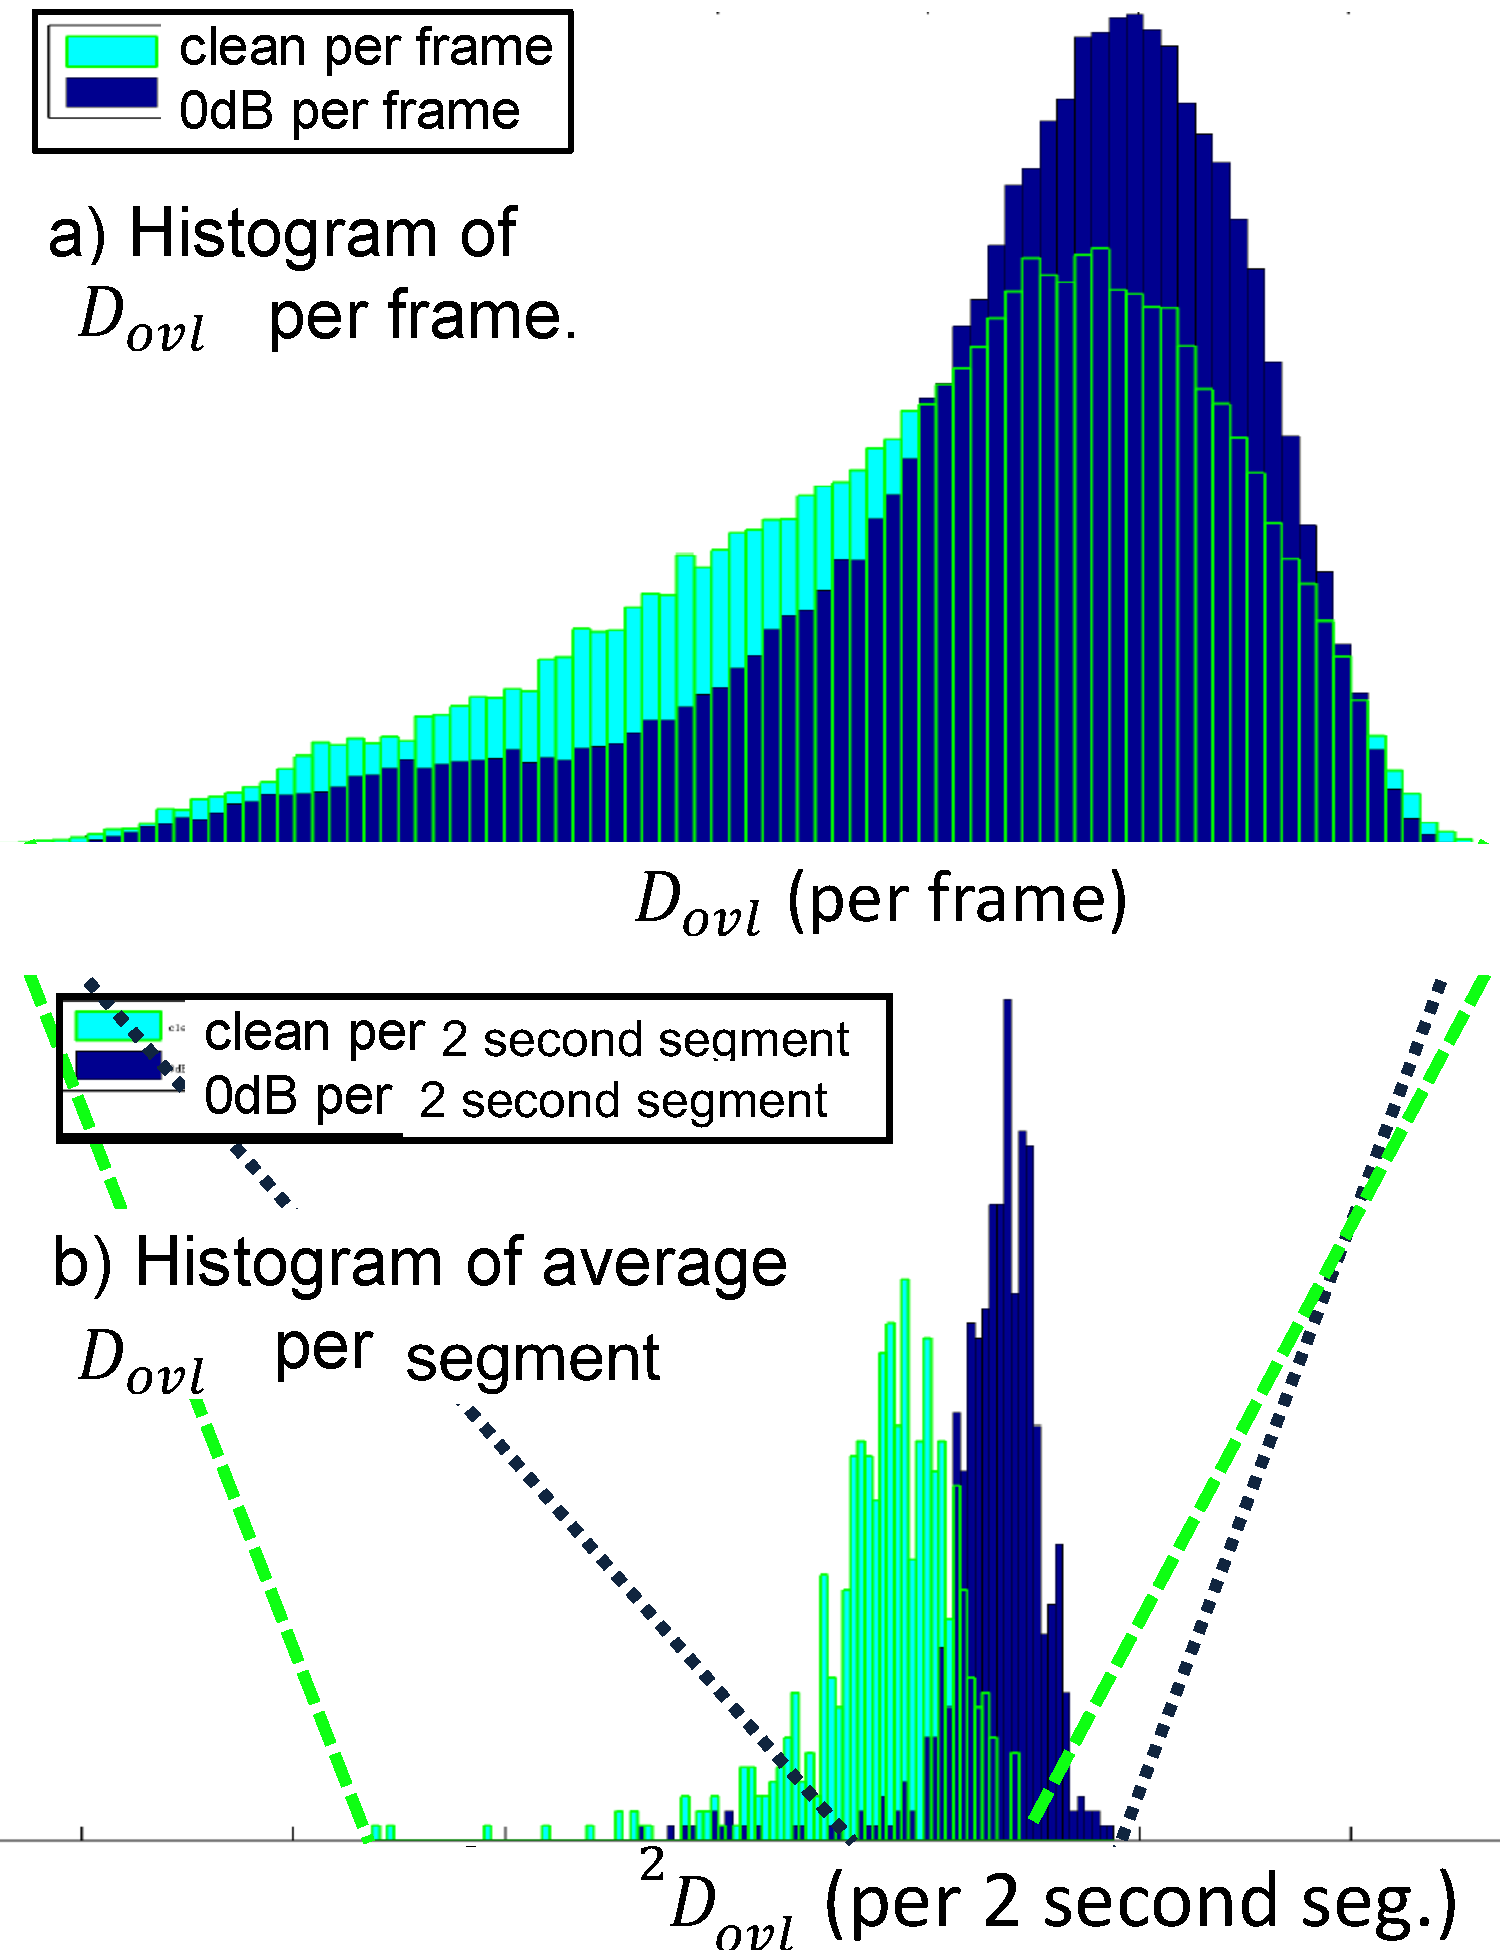
\includegraphics[height = 3in, width=0.4\textwidth]{figures/compare_pframe_pseg_hists}
	\vspace{-1mm}
	\caption{\it The effect of ensemble decisioning on distinguishability of overlapped regions. a) shows score per frame histograms and b) shows the histogram of ensemble scores. Using multiple frames to make a decision helps separate the distributions of clean and overlapped segments.}
	\vspace{-2mm}
	\label{fig:compare_perframe_and_perfile_ovldethist}
\end{figure}

The observation in Fig.~\ref{fig:compare_perframe_and_perfile_ovldethist} a characteristic of all non-stationary interferences, that frame-level detection is significantly less reliable compared to ensemble decisions. 
Therefore, longer durations should be used to detect the presence of overlap. 
Section~\ref{sssec:ovl_frame_vs_seg} will investigate the relation between segment lengths (in other words, number of frames) and detection performance. 
%\subsection{HMM-based harmonic tracking for overlap detection}
%A more elaborate setup to track harmonic trajectories involves using a hidden Markov model (HMM) to model Pyknogram patterns. This allows for a supervised classification of speech segments into overlap and single-speaker speech. To do so, we propose using an initial segmentation of a given audio stream based on the Bayesian Information Criterion (BIC segmentation)~\cite{BIC}. The shorter segments are then compared against two pre-trained HMMs, one for overlapped and the other for single-speaker speech. The initial BIC segmentation is to allow for detection on shorter segments, since overlapped speech is considerably less frequent in a conversation compared to the total amount of speech. The combination of BIC segmentation and HMM-based classification allows for a practical overlap detection mechanism that fits well with analyzing conversations recorded in real conditions (as opposed to artificial datasets with simulated overlaps). Among other benefits of this framework is its compatibility with speaker diarization tools in which overlapped speech is considered a nuisance (see Sect.~\ref{sec:intro}). 


%\subsection{Pyknogram Analysis in Overlap}
%
%Now that we have chosen a representation for our signal, we would like to analyze its behavior at overlapped regions. 
%A reasonable way to approach this would be to have a close-up look at Pyknograms to confirm whether they follow the same trend mentioned in Sec.~\ref{sssec:pykno_select}. 
%This is accomplished by calculating Pyknograms of segmented phones overlapping each other. 
%The outcome of this analysis will provide insight in developing an overlap detection strategy. 
%
%\subsection{Pyknograms in Voiced Phonemes}
%
%The most important group of overlapped pairs are voiced-voiced combinations, phonemes in which foreground and background speech contains harmonic structures.
%From a practical point of view, voiced speech is more likely to demonstrate distinguishable patterns during overlaps. 
%In addition, vowels and in general voiced speech contain more useful spectral content for speaker recognition~\cite{hansen2015SIDmagazine}, which is one of the pinnacles of this study. 
%To compare the behavior of Pyknograms at single-speaker and overlapped speech segments, a series of artificial overlapped segments are created from TIMIT data. 
%These segments are overlapped by phones from different speakers. 
%To investigate the effect of energy levels, a range of signal-to-interference (SIR) values from $0dB$ (most overlapped) to $100dB$ (single-speaker) is used. 
%
%Take the phone /\textscripta/, for example. By creating all the combinations of overlaps with this phone, we  see how the Pyknogram spectra are affected (Fig.~\ref{fig:overlapped_pykno_aa}).
%
%The comparison will be between single-speaker /\textscripta/ (spoken by male speakers), compared with /\textscripta/ overlapped by three groups of phonemes (also from male speakers). 
%The overlapping phones are: 
%\begin{itemize}
%	\item Front-Vowels (/i\textlengthmark/,/\textsci/,/e/,/\ae/)
%	\item Mid-Vowels (/\textscripta/,/\textrhookrevepsilon/,/\textturnv/,/\textopeno/)
%	\item Back-Vowels (/u/,/\textscu/,/o/)
%	\item Diphthongs (/\textscripta\textsci/,/\textopeno\textsci/,/\textscripta\textscu/,/e\textsci/,/o\textscu/,/ju/)
%	\item Semivowels (/w/,/l/,/r/,/y/)
%	\item Nasal Consonants (/m/,/n/,/$\eta$/)
%	\item Other Consonants (except nasals)
%\end{itemize}
%
%Nasals have been separated from the list above due to their significant role in speaker identification. Figure~\ref{fig:overlapped_pykno_aa} shows that cross-frequency dimension of Pyknograms tends to become more flat as overlapped framed are introduced. 
%Such behavior is also observed in the autocorrelation spectra~\cite{sapvr_paper}. 

\newpage

\subsection{Evaluation}
\label{ssec:exp_pykno}

This section evaluates the proposed pyknogram-based overlap detection system in terms of {\it accuracy, robustness,} and {\it precision}. 
Evaluation tasks for each SIR category are in the form of standard binary classification problems, where target examples are from a collection of overlapped signals with fixed SIR values and non-target signals are clean (single-speaker). 
This section measure system performance using detection equal error-rates (EER; where false-positive and false-negative errors are equal). 
EER values are presented in Fig.~\ref{fig:ovl_det} for different SIRs. 
The expectation is that the detection algorithm should be consistent across a range of SIR values (i.e. robustness). 
As for precision, we are interested to know how short signals can be before overlap detection performance significantly drops (noting the observation in Fig.~\ref{fig:compare_perframe_and_perfile_ovldethist}). 


\vspace{3mm}
\subsection{Overlapped speech detection vs. SIR (Robustness \& Accuracy)}
\label{sssec:ovl_frame_vs_sir}
\begin{figure}[b!]
	\centering
	\hspace{-1mm}
	\textbf{Overlap Detection vs. SIR}\par\medskip
	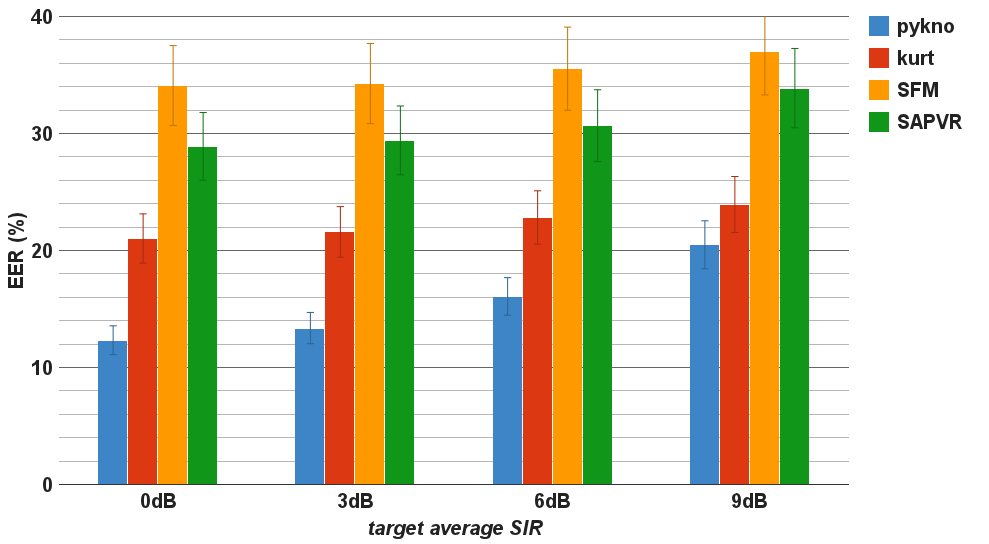
\includegraphics[height = 3.1in, width=0.7\textwidth]{figures/ovldet_vs_sir}
	\vspace{-1mm}
	\caption{\it Overlap detection EER for different SIR values. The higher the SIR, the more difficult it is to detect the presence of interfering speakers.}
	\vspace{0mm}
	\label{fig:ovl_det}
\end{figure}
Here the performance of pyknogram-based overlap detection is compared with the three baseline algorithms (mentioned in Sect.~\ref{ssec:baseline}) across different SIR values. 
The goal is to monitor the chances in EER as SIR values increase. 
The experiments are designed to compare features in terms of how much separation they can create between single-speaker from overlapped speech. 
Overlapped signals are defined as target and single-speaker signals (i.e., clean) are defined as non-target. 
The task is to perform binary classification using feature values as scores. 
The target/non-target signals used in this binary classification task are obtained from a pool of overlapped and single-speaker files. 
This task is repeated for each SIR condition separately to monitor the impact of SIR. 
In each task, overlapped signals with the same SIR are used as target examples and the overlap detection score (or feature value) assigned to them is compared against the scores estimated for clean files to compute the binary classification EER. 
Figure~\ref{fig:ovl_det} compares performances for the proposed and baseline systems across SIR values of $0, 3, 6$ and $9dB$. 
Pyknograms are shown to provide lower EER over the baseline features. 
This robust behavior across different SIR values is due to the resonance enhancement process, which takes place during Pyknogram extraction. 
Enhancing resonances reduces false alarm detections by removing the effects of non-harmonic components. 
These non-harmonic components are known to be confusing to overlap detection systems. 


%\begin{figure}[!t]
%\centering
%\hspace{-1mm}
%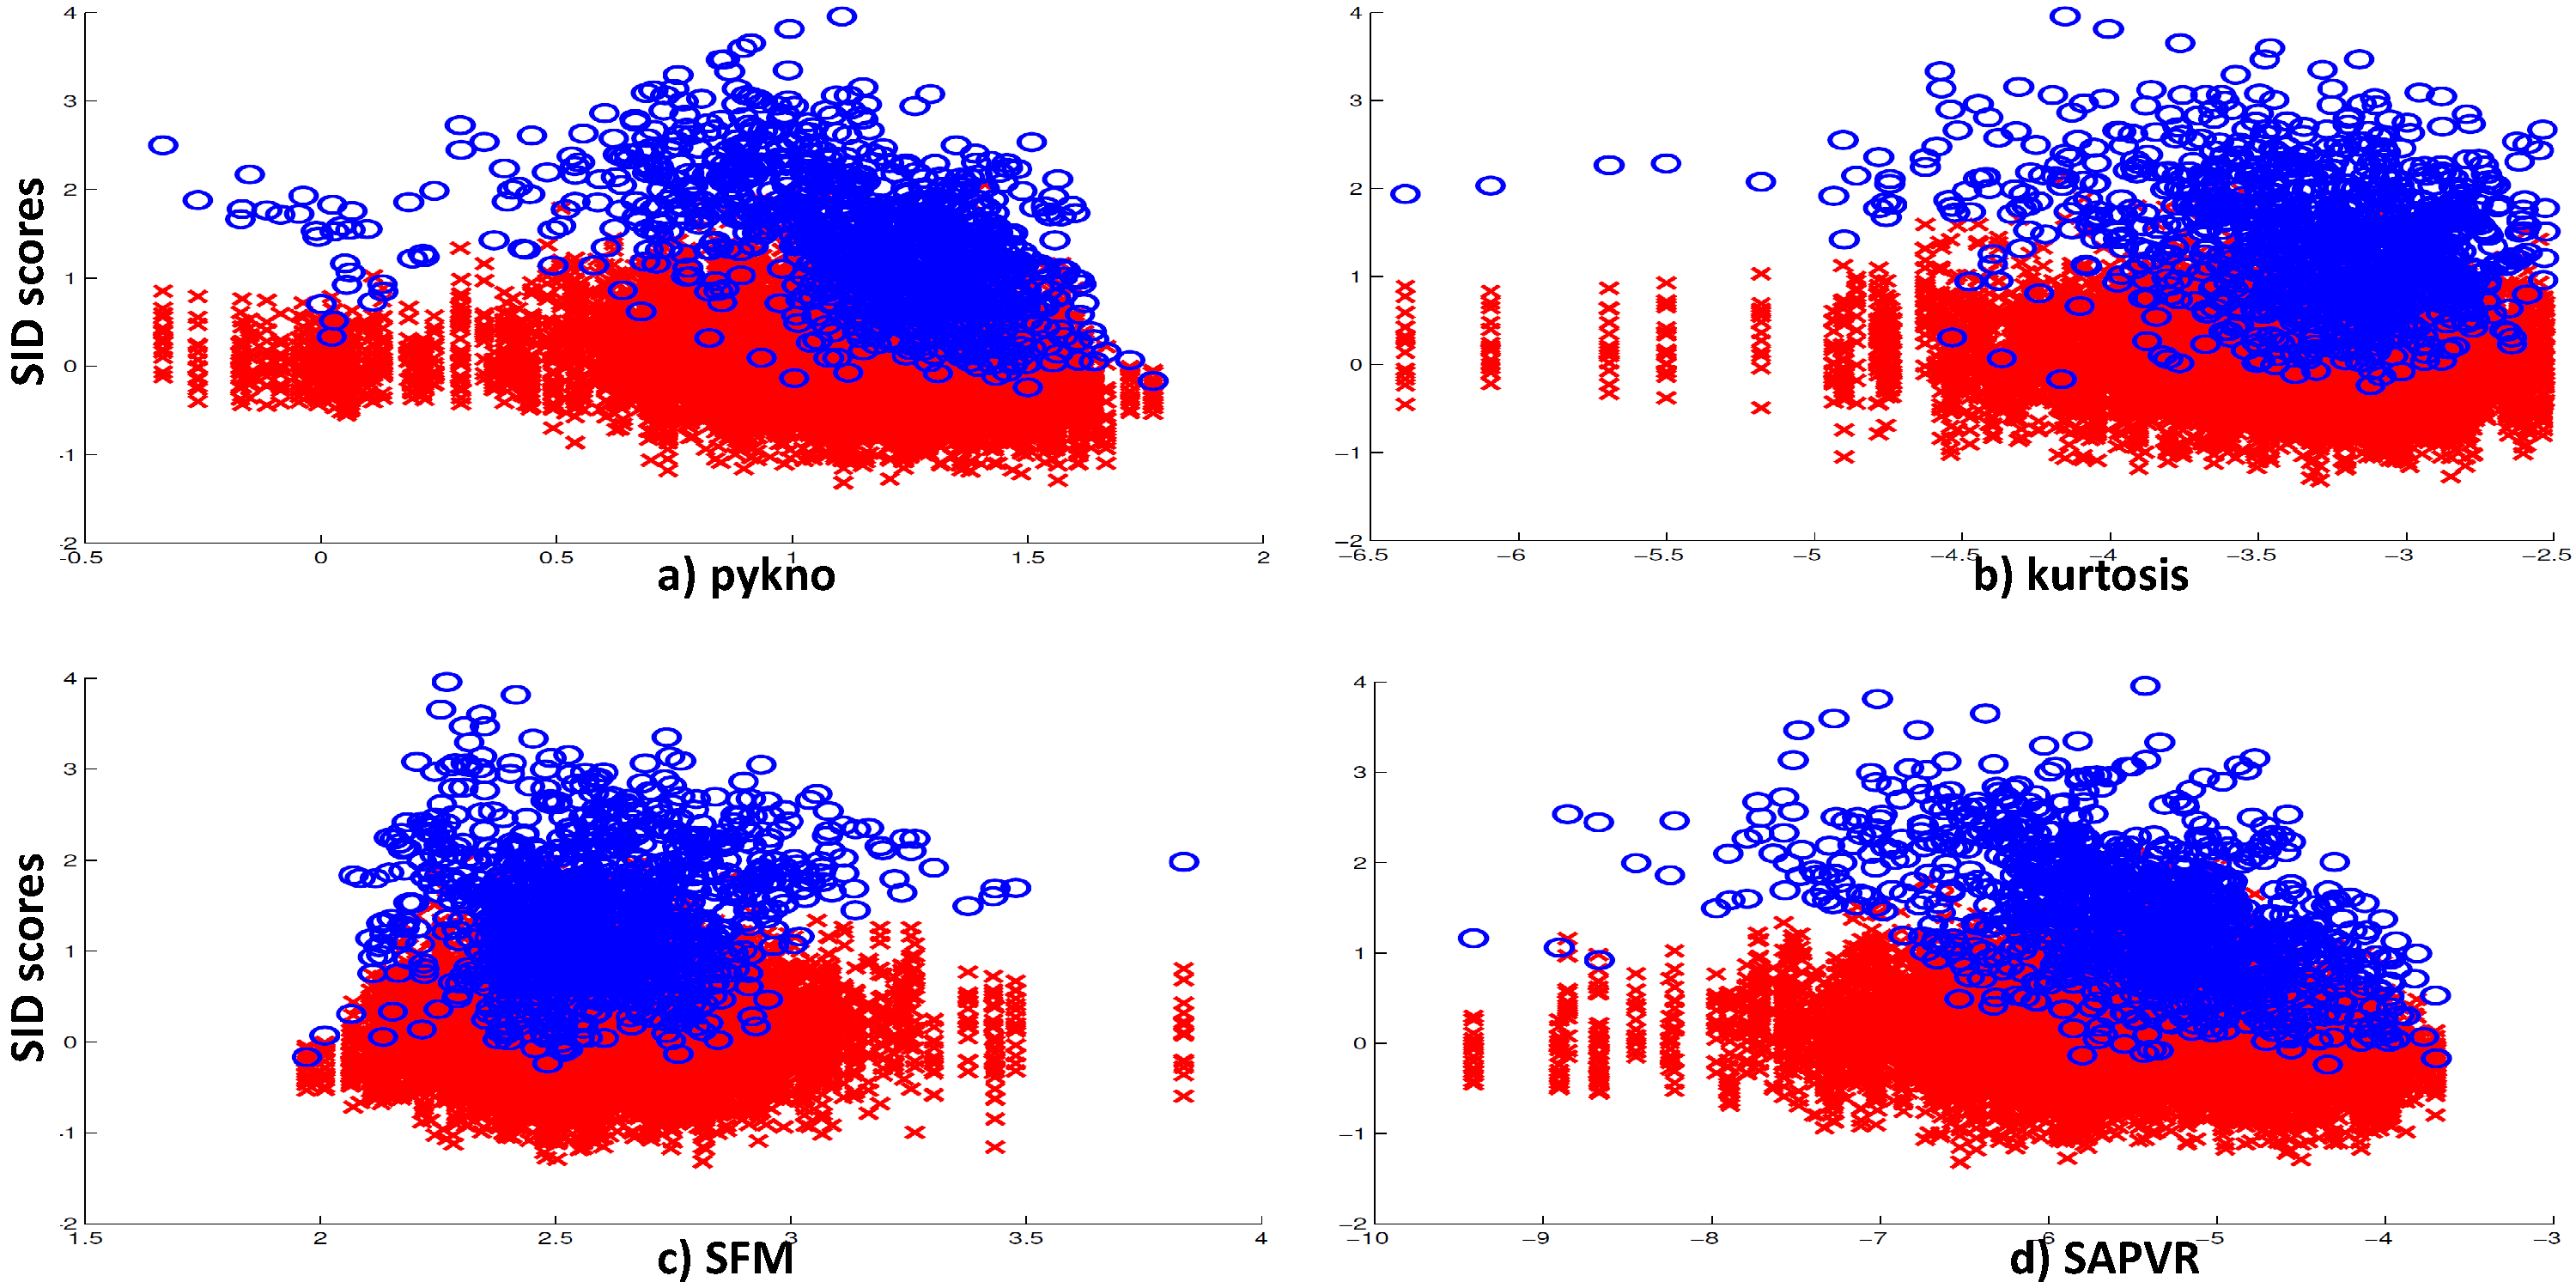
\includegraphics[height = 3.5
%in, width=1\textwidth]{figures/sid_ovl_scatterplots}
%\vspace{-3mm}
%\caption{\it 2-dimensional score-space with SID scores on the y-axis and overlap detection scores on the x-axis. Each plot is with respect to one of the overlap scores. Blue circles ($\bigcirc$) represent target and red crosses ($\times$) represent imposter trials. (b) shows log-kurtosis for better visualization.}
%\vspace{-3mm}
%\label{fig:q_stack_scores}
%\end{figure}


\subsection{Overlapped speech detection vs. segment length}
\label{sssec:ovl_frame_vs_seg}

A main concern in dealing with overlapped regions is that overlap decisions are less reliable as segment lengths become shorter. 
This restricts algorithm precision in terms of the ability to detect overlap in a frame-based framework. 
It was shown in Sect.~\ref{ssec:unsupervised_ovl_det_pykno} that using multiple adjacent frames in the form of average $D_{ovl}$ (i.e., $^MD_{ovl}$) increases separability between single-speaker and overlapped speech distributions. 
The averaging defined in (\ref{eq:seg_dovl}) can be applied to our baseline features. 

This method of treating non-stationary signals can help define the ``precision'' of proposed overlap detection algorithms. 
In other words, the question becomes: ``what is the least number of frames required to maintain stable detection accuracy?'' 

\begin{figure}[h!]
	\centering
	\hspace{-1mm}
	\textbf{Precision of Overlap Detection methods}\par\medskip
	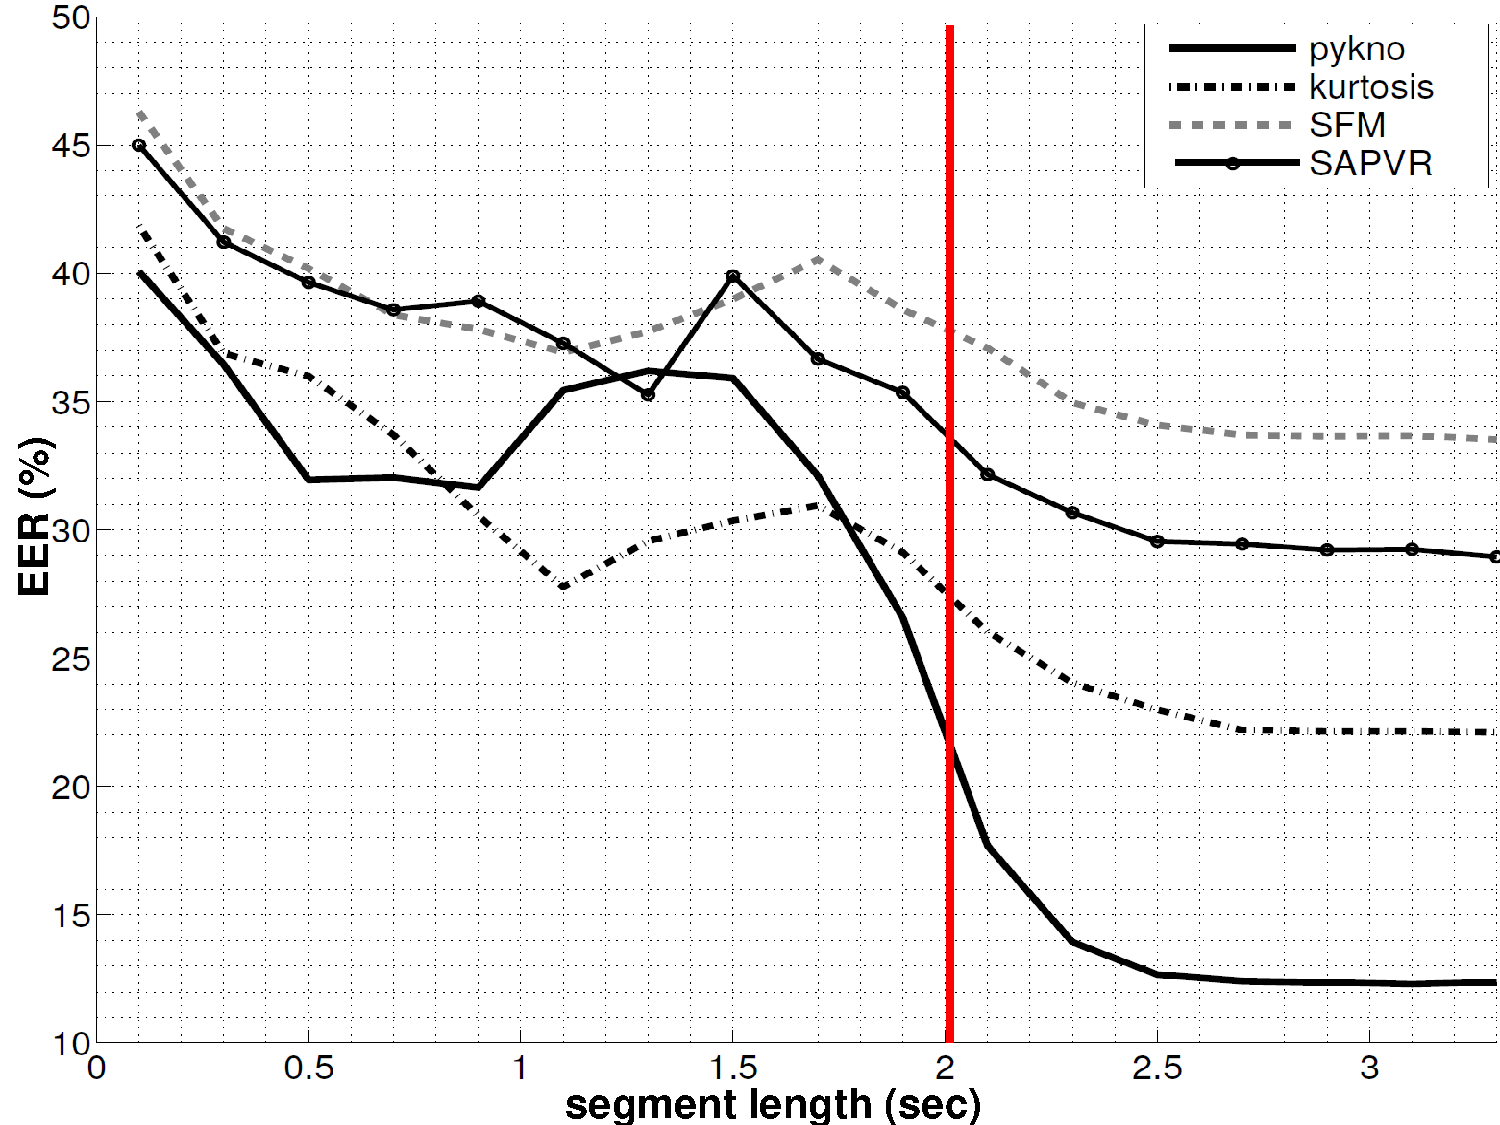
\includegraphics[height = 3.1in, width=0.5\textwidth]{figures/eer_vs_time}
	\vspace{-1mm}
	\caption{\it Overlap detection EER as a function of segment length. The plot shows that signal lengths should be at least $2$ seconds for the algorithms to start reaching their best performance.}
	\vspace{0mm}
	\label{fig:ovl_det_precision}
\end{figure}


Precision is most valuable in tasks such as speaker diarization in conversational speech, where overlap mostly occurs at speaker transitions in turn-takings. 
The goal of this analysis is to evaluate system precision and compare pyknogram-based detection with baseline features. 
It is useful to see how short can overlap segments get before observing a significant drop in system performance. 
Once again, overlap detection performance is measured through the detection EER. 
Figure~\ref{fig:ovl_det_precision} shows the change in system performance as shorter duration segments are used to obtain overlap decisions. 
It is shown that regardless of the feature used to detect overlaps, performance drops as fewer frames (shorter time segments) are used to make decisions. 
Furthermore, we see that performance stabilizes for all features for segments 2 seconds and longer. 


\newpage
\section{Gammatone Sub-band Frequency Modulation Spectra}
\label{sec:ch2_GSFM}
So far, one of the two proposed overlap detection methods has been presented. 
The second method discussed in this chapter provides an alternative way of viewing overlapped speech. 
The theory and motivation behind the second proposed feature extraction are described in this section. 

\subsection{Motivation}

\begin{figure}[b!]
	\centering
	\hspace{-1mm}
	\textbf{single and dual tone FM spectra}\par\medskip
	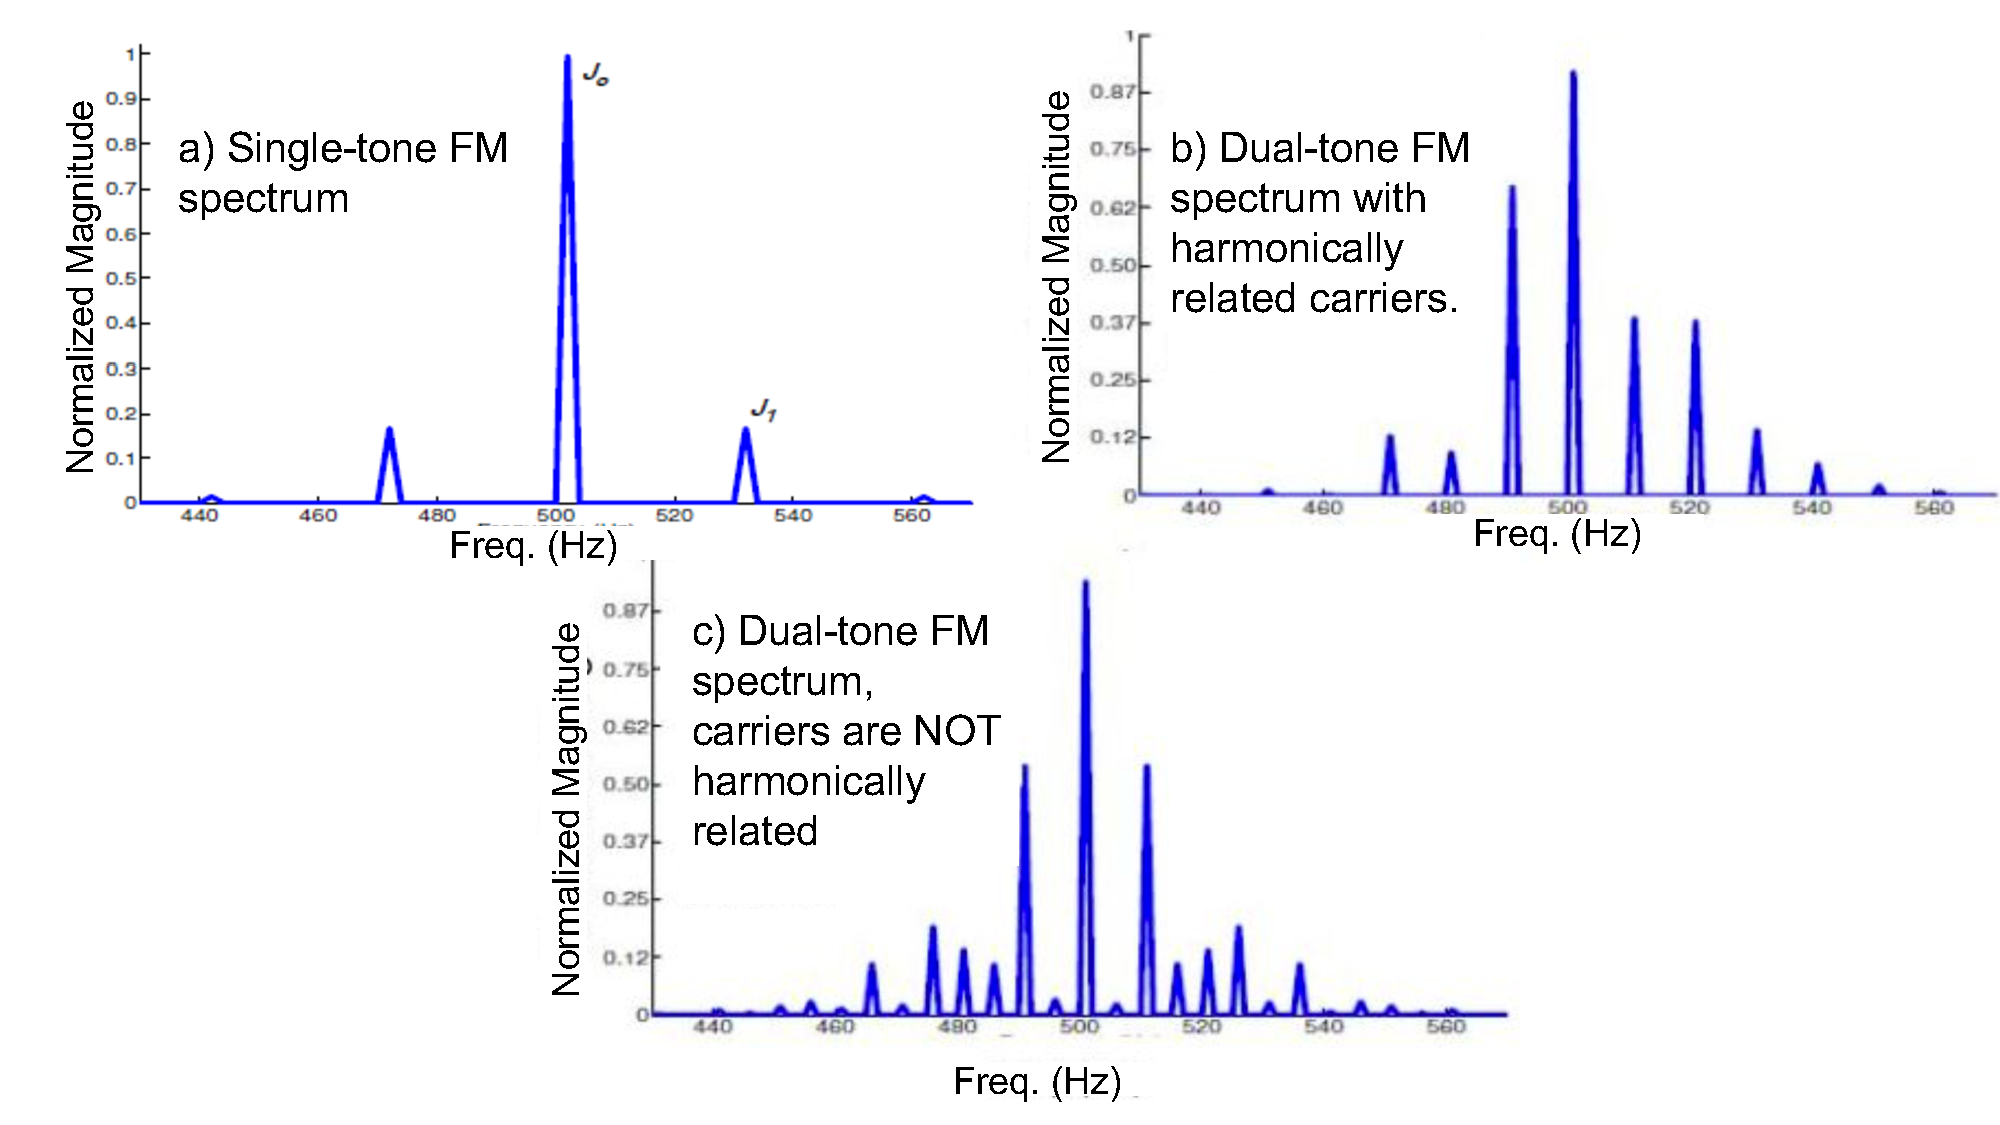
\includegraphics[height = 3.1in, width=0.8\textwidth]{figures/tone_FM_spectra}
	\vspace{-1mm}
	\caption{\it Comparing the dispersity of different FM signals.
		From top to bottom. 
		a) Single-tone FM Spectral Magnitude $f_1$ = 10. 
		b) Harmonically related double-tone FM Spectral Magnitude $f_1$=10, $f_2$=20. 
		c) Not harmonically related double-tone FM Spectral Magnitude f1=10, f2=25}
	\vspace{0mm}
	\label{fig:tone_fm_spectra}
\end{figure}

This section begins with a brief analysis of frequency modulated (FM) sinusoids and their spectral characteristics. 
Modulating the frequency of a sinusoid results in a signal with more frequency components than the original sinusoid. 
For example, the spectrum of a single-tone frequency modulated carrier contains frequency components that depend both on the amplitude and frequency of the modulating signal, both of which contribute to the modulation index, $\beta$~\cite{carlson2010communication}. 
Fig.\ref{fig:tone_fm_spectra}-a shows the spectrum of a single-tone FM signal. 
This signal is typically simplified and defined as, 

\begin{equation}
\label{eq:1sin_fm}
x_c(t) = A_ccos(2\pi f_ct+(\beta sin(2\pi f_mt))),
\end{equation}
where $f_m$ is the frequency of the modulating sinusoid and $A_c$ and $f_c$ are the carrier amplitude and frequency, respectively. 
In Fig.\ref{fig:tone_fm_spectra}-a, the amplitude of the $n^{th}$ frequency component of $x_c(t)$, considering $f_c$ as the origin, is the $n^{th}$ order Bessel coefficients at $\beta$ (i.e., $J_n(\beta)$). 

Since overlapped speech consists of two speech signals, a closer analogy to the problem of overlapped speech is observed in the case where the modulating signal has more than one sinusoid (as seen in Eq.(\ref{eq:2sin_fm})). 
Fig.\ref{fig:tone_fm_spectra}-b~and~-c compare the spectra of double-tone FM signals in two scenarios. 
In Fig.\ref{fig:tone_fm_spectra}-b, the two tones are harmonically related (one is an integer multiple of the other), while in Fig.\ref{fig:tone_fm_spectra}-c, the frequencies of the modulating tones do not share a common integer factor. 
Consequently, the spectrum in Fig. \ref{fig:tone_fm_spectra}(c) is more disperse than that in Fig.\ref{fig:tone_fm_spectra}-b. 
The same conclusion can be made from Eq.(\ref{eq:2sin_fm_bessel}) where the number of frequency components of the Fourier transform of $x_c(t)$ is greater when $f_1$ and $f_2$ are not harmonically related. 
An FM signal for a double-tone modulating signal with frequencies $f_1$ and $f_2$ can be represented as,
\begin{equation}
\label{eq:2sin_fm}
x_c(t) = A_ccos(2\pi f_ct+[\beta_1 sin(2\pi f_1t) + \beta_2 sin(2\pi f_2t)]).
\end{equation}

Defining $J_n(.)$ as the nth order Bessel function, the Fourier series expansion of Eq.(\ref{eq:2sin_fm}) can be compactly defined as follows, 
\begin{equation}
\label{eq:2sin_fm_bessel}
x_c(t) = A_c\sum\limits_n\sum\limits_m J_n(\beta_1)J_m(\beta_2)cos(2\pi (f_c+nf_1+mf_2)t).
\end{equation}

This observation is particularly interesting, since in overlapped speech segments one of the major confusions is in distinguishing related harmonics (i.e. those that belong to the same speaker) versus non-related harmonics. 
Here, Eq.(\ref{eq:2sin_fm_bessel}) suggests that the number of frequency components of $x_c(t)$ in a given range is greater when caused by non-harmonically related frequencies. 
On the other hand, if $f_1$ and $f_2$ are harmonically related, (\ref{eq:2sin_fm_bessel}) can be simplified as, 
\begin{equation}
\label{eq:2sin_fm_bessel_simplified}
x_c(t) = A_c\sum\limits_{n^\prime} K_{n^\prime}cos(2\pi (f_c + n^\prime f_1)t),
\end{equation}
where $n^\prime$ is defined such that for each $m$ and $n$ pair,
\begin{equation}
\label{eq:knprime}
K_{n^\prime} = J_n(\beta_1)J_m(\beta_2). 
\end{equation}


\subsection{GSFM system description}
Despite analyses on sinusoidal signals, a substantial difference between the spectral characteristics in multi-tone and single-tone FM signals versus speech is that in speech the spectrum consists of multiple harmonic components across its bandwidth. 
In order to interact with only a few sinusoidal components, a natural solution is to decompose the signals into multiple sub-bands by means of a filter-bank. 
As was the case for Pyknograms in Sect.~\ref{ssec:pykno_estimate}, a gammatone filter-bank is used for sub-band analysis\footnote{The gammatone filter-bank has been widely used in computational auditory scene analysis (CASA) literature to simulate the auditory periphery processing.}. 
Sub-band outputs are used to modulate the instantaneous frequency of a sinusoidal carrier. 
Detecting overlapped speech with the use of multiple sub-bands results in multiple decisions for each speech segment. 
If a specific channel does not have the sufficient information to distinguish overlapped speech from single-speaker speech, the lack of information can be compensated by other sub-bands. 
This framework results in a more consistent detection compared to a scenario where the system only relies on a single decision per frame. 
The feature extraction procedure is summarized in Fig.~\ref{fig:gsfm_block_diagram}:

\begin{enumerate}
	\item apply a gammatone fiterbank to the speech signal
	\item demodulate each sub-band to base-band (since the output for each channel is a band-pass signal and located around the center frequency of each sub-band). 
	This is done by	multiplying a sinusoid tuned at the center frequency of	the gammatone sub-band followed by low-pass filtering.
	\item Block the output signals into frames. 
	\item Compute the frequency modulated signal for each time-frequency unit by using the output of the previous step as the modulating signal. 
	\item Use the spectral magnitude of the modulated signal as the output.
\end{enumerate}

\begin{figure}[t!]
	\centering
	\hspace{-1mm}
	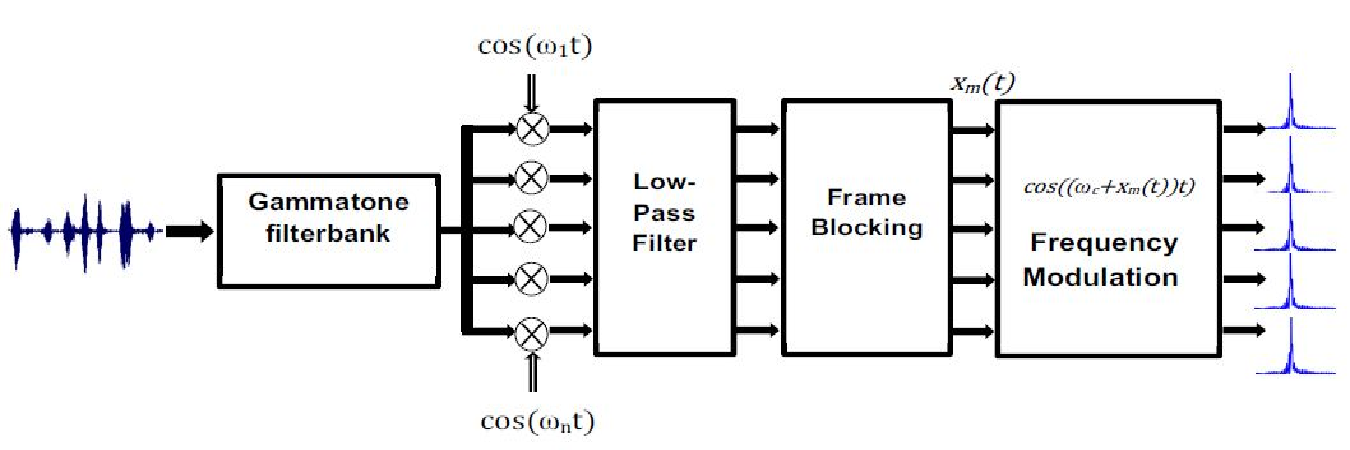
\includegraphics[height = 2.5in, width=1\textwidth]{figures/gsfm_block_diagram}
	\vspace{-1mm}
	\caption{\it GSFM block diagram.}
	\vspace{0mm}
	\label{fig:gsfm_block_diagram}
\end{figure}

Given the output gammatone sub-band frequency modulated (GSFM) spectra, many operations could be used to quantify the amount of dispersion. 
A technique similar to that proposed in~\cite{sapvr_2000} is to use the relative peak amplitudes in GSFM spectra. 
As shown in Fig.~\ref{fig:tone_fm_spectra}, the amplitudes of Bessel components drop
more rapidly for harmonically related tones and even more so for single tones. 
The relative peak amplitude ratios can be used represent spectral roll-off in the FM spectra for each time-frequency unit. 

\begin{figure}[h!]
	\centering
	\hspace{-1mm}
	\textbf{GSFM roll-off}\par\medskip
	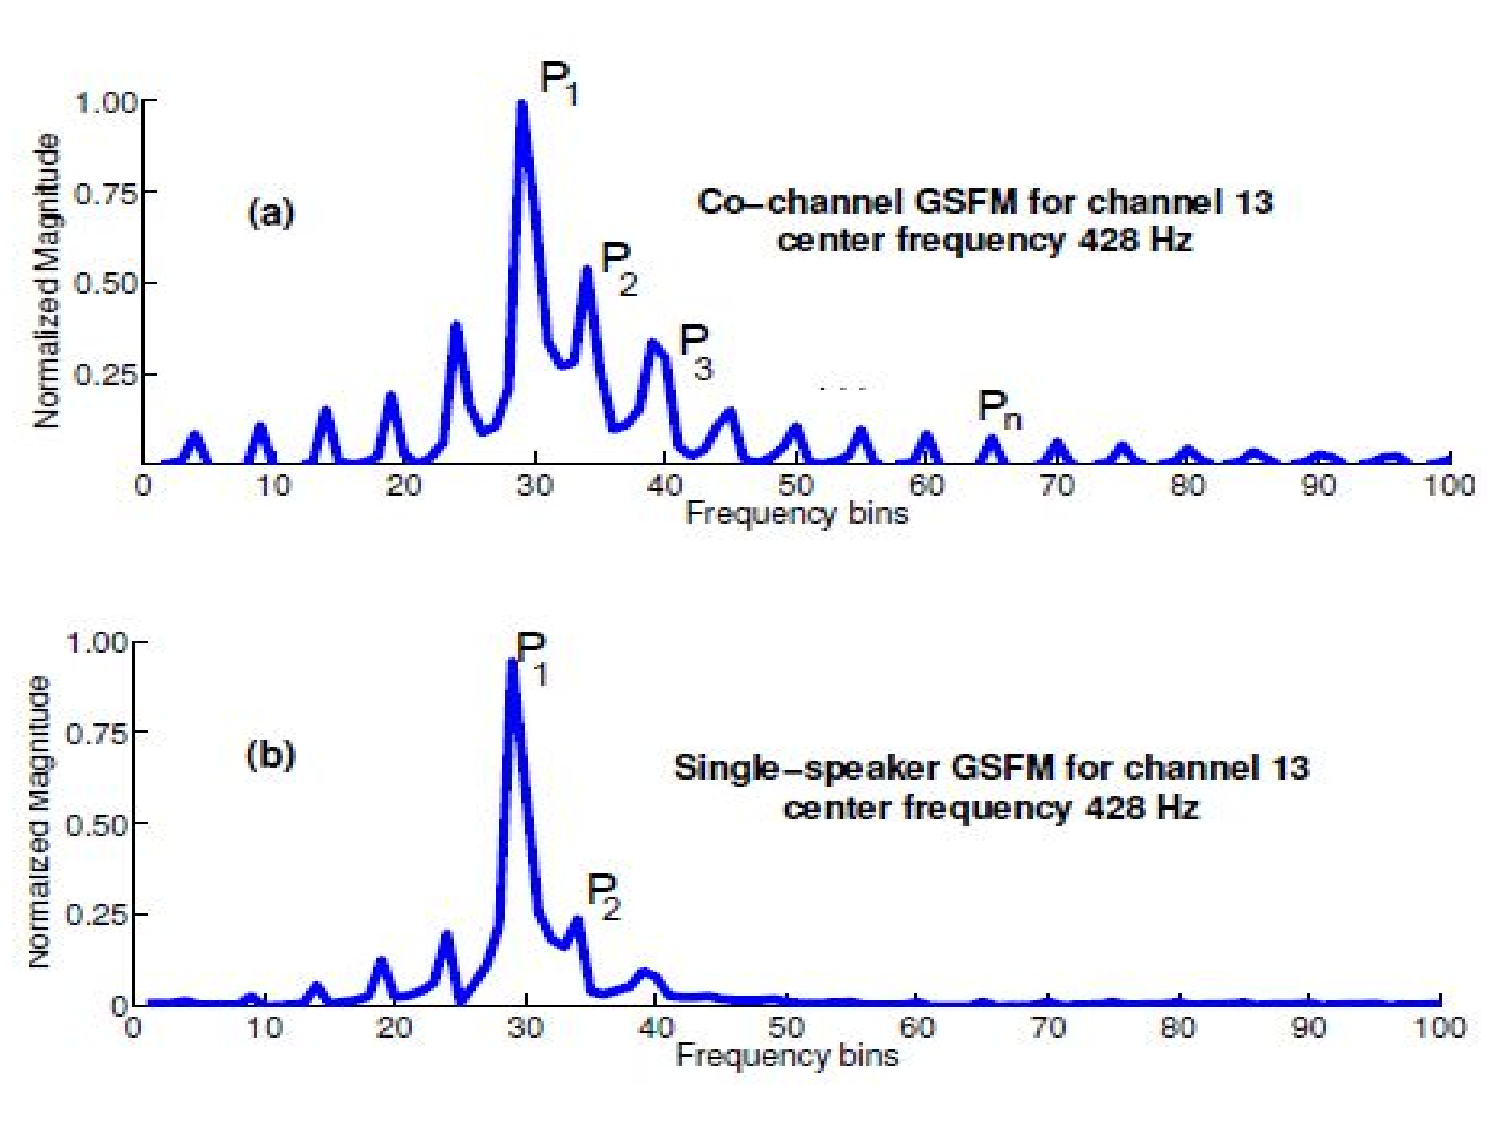
\includegraphics[height = 2.8in, width=0.6\textwidth]{figures/gsfm_rolloff}
	\vspace{-1mm}
	\caption{\it Comparison of GSFM spectra for overlapped speech and single-speaker speech. a) The GSFM of an overlapped speech segment at the 13th gammatone sub-band with center frequency 428 Hz. b) The GSFM of single-speaker speech at the same sub-band.}
	\vspace{0mm}
	\label{fig:gsfm_rolloff}
\end{figure}

Figure~\ref{fig:gsfm_rolloff} shows the difference in GSFM spectra for a typical time-frequency unit, $(t,i)$, in overlapped and single-speaker speech. 
GSFM roll-offs are defined as: 
\begin{equation}
\label{eq:gsfm_rolloff}
R(t,i) = \sum\limits_{k=2}^{N} \frac{P_1(t,i)}{P_k(t,i)}
\end{equation}
where $t$ and $i$ respectively denote the frame and sub-band indexes. 
$P_k(t, i)$ corresponds to the $k^{th}$ peak in the GSFM spectrum with respect to the center peak (i.e., $P_1(t,i)$) that lies on the carrier frequency and is equal to the 0th Bessel coefficient (see Fig.~\ref{fig:gsfm_rolloff}). 
We call $R(t, i)$ the GSFM roll-off factor computed at T-F unit $(t, i)$. 
The collection of GSFM roll-off factors are used as a time-frequency representation for any given speech segment. 


\subsection{Unsupervised overlap detection using GSFM roll-off}
\label{sssec:unsupervised_ovl_det_gsfm}
The feature used to detect overlapped speech uses a combination of the information obtained from all sub-bands, since each band can provide a local decision as to whether a frame contains speech from more than one speaker. 
We use the overall count of highly disperse time-frequency units (i.e., units with higher GSFM roll-off) per time unit as a decision score for the amount of overlapped speech in a given speech segment. 
Highly disperse roll-off values are obtained by applying a 2 class K-means clustering. 
K-means results in a threshold of the roll-off values, $R_{thr}$. 
By applying the threshold to the GSFM roll-off values (i.e. $R(t, i)$) for a given speech segment, one can estimate the decision score for overlapped speech detection. 
The decision score is calculated using the following equation:
\begin{equation}
\label{eq:gsfm_features}
S = \frac{1}{T}\sum\limits_{\forall (t,i)} I\{R(t,i) > R_{thr}\}
\end{equation}
where
\begin{equation}
I\{x\}=\begin{cases}
1, & \text{if x is true}.\\
0, & \text{otherwise}.
\end{cases}
\end{equation}

Here, T is the signal length in time units and $R_{thr}$ is the GSFM threshold obtained from clustering GSFM roll-off values into two sets, corresponding to higher and lower values. 
The more the number of high roll-off values per unit time, the higher the likelihood of overlapped speech. 

\subsection{Evaluation}
\label{ssec:exp_gsfm}
Overlap detection experiments for GSFM are conducted in a manner similar to what was presented in Sect.~\ref{ssec:exp_pykno}. 
Once again, it is useful to investigate features in terms of accuracy, robustness, and precision. 

\vspace{3mm}
\subsection{Overlapped speech detection vs. SIR (Robustness \& Accuracy)}
\label{sssec:ovl_frame_vs_sir_gsfm}
\begin{figure}[b!]
	\centering
	\hspace{-1mm}
	\textbf{Overlap Detection vs. SIR}\par\medskip
	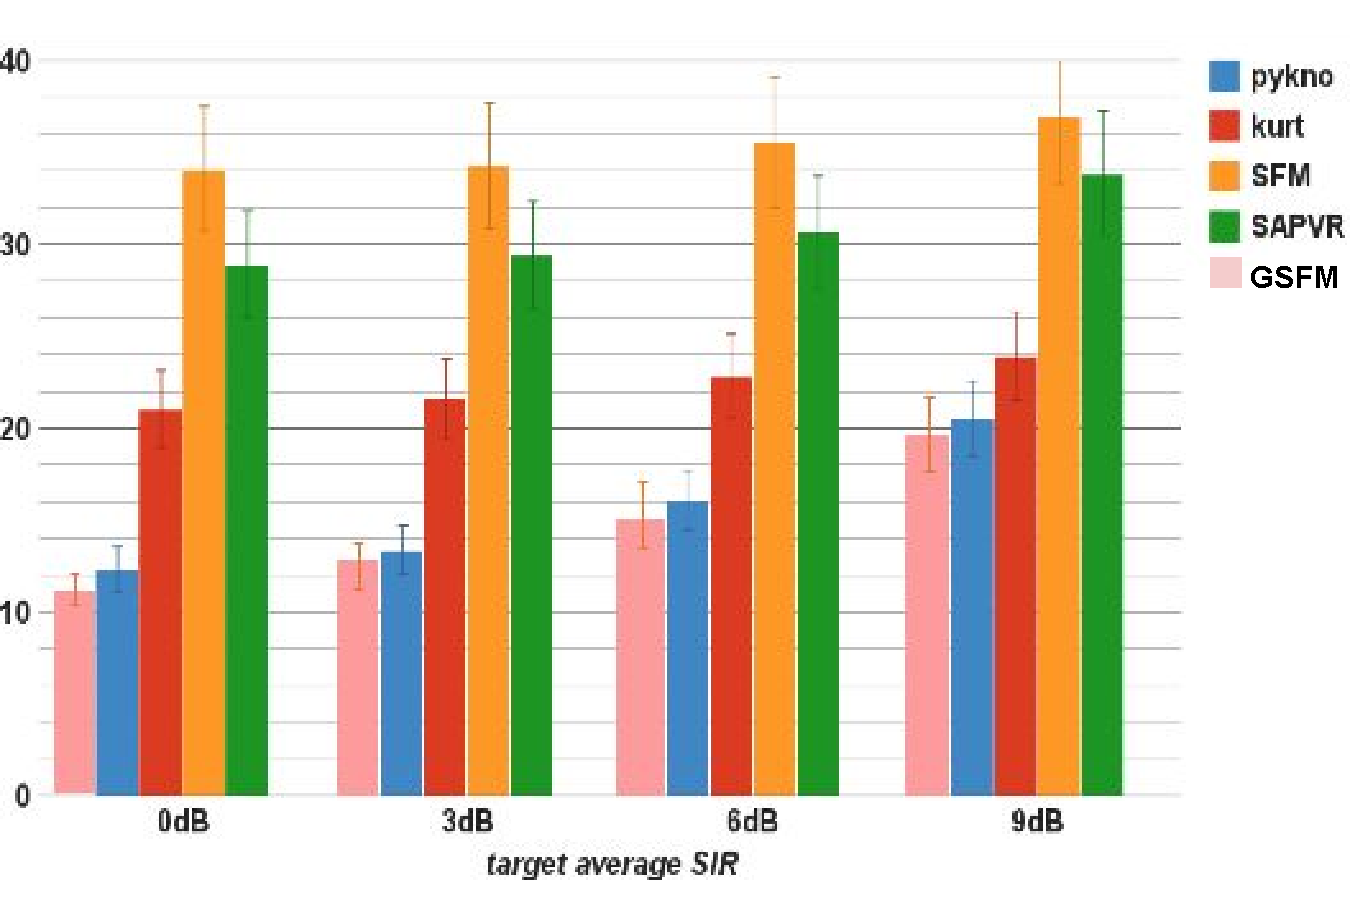
\includegraphics[height = 3.1in, width=0.7\textwidth]{figures/ovl_det_vs_sir_gsfm}
	\vspace{-1mm}
	\caption{\it Overlap detection EER for different SIR values. The higher the SIR, the more difficult it is to detect the presence of interfering speakers.}
	\vspace{0mm}
	\label{fig:ovl_det_gsfm}
\end{figure}

As explained before, a main challenge in overlap detection is addressing a large range of interference ratios, even within a single recording. 
Ideally, an overlapped speech detection system should perform consistently well in any SIR. 
However, this is neither feasible nor necessary. 
As mentioned earlier, the database used in this study consists of 4 different absolute SIR conditions. 
Figure~\ref{fig:ovl_det_gsfm} compares the performance of the proposed GSFM spectral roll-off feature with Pyknogram-based and baseline features.

\subsection{Overlapped speech detection vs. segment length}
\label{sssec:ovl_frame_vs_seg_gsfm}
All overlap detection algorithms presented in this study use the collective knowledge obtained from multiple adjacent time frames from a given speech segment to estimate a score that represents the likelihood of overlapped speech. 
The precision of the overlap detection system tells us how short a segment could be before we observe a substantial drop in performance. 
In Fig.~\ref{fig:ovl_det_precision_gsfm}, EER across different signal time lengths in 0dB average SIR. 
It is observed in Fig.~\ref{fig:ovl_det_precision} that the EER varies most in kurtosis for different signal durations. 
This is expected, since kurtosis is calculated from $3^{rd}$ and $4^{th}$ order moments, which are less accurately estimated with insufficient data. 
From Fig.~\ref{fig:ovl_det_precision_gsfm}, we also conclude that the breaking point for all systems is at approximately 2 seconds, which implies that overlap detection performance drops dramatically for segments less than 2 seconds long. 
The performance drop is more severe for GSFM features, since it uses the distribution of roll-off values in calculating the final score (\ref{eq:gsfm_features}). 

\begin{figure}[h!]
	\centering
	\hspace{-1mm}
	\textbf{Precision of Overlap Detection methods}\par\medskip
	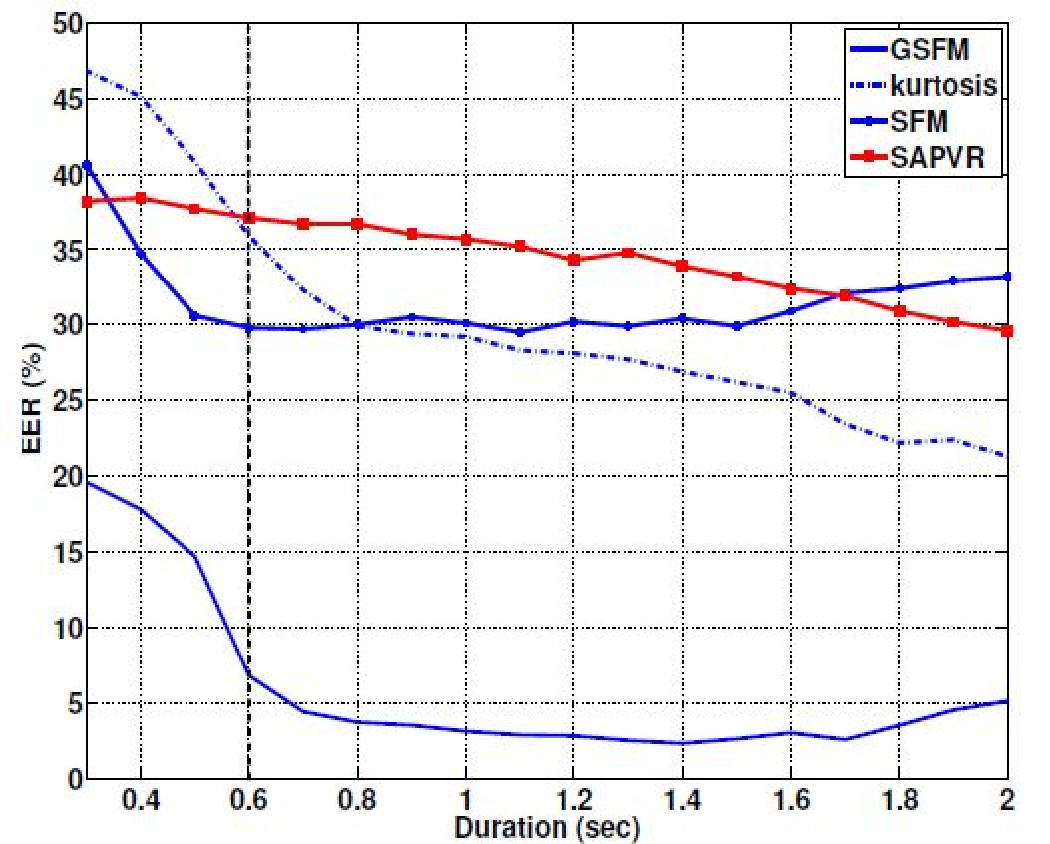
\includegraphics[height = 3in, width=0.5\textwidth]{figures/eer_vs_time_gsfm}
	\vspace{-1mm}
	\caption{\it Overlap detection EER as a function of segment length. }
	\vspace{0mm}
	\label{fig:ovl_det_precision_gsfm}
\end{figure}

\newpage
\section{Pyknogram vs. GSFM}
\label{sec:ch2_Pykno_vs_GSFM}
Typical overlap detection systems are designed to detect overlapped speech segments in data that are generally clean of any environment noise, which makes them less reliable for data collected in real meeting and conversation scenarios. 
This section investigates the scenario in which overlap detection takes place in noisy conditions. 
In other words, in addition to speaker interference, environment noise is also present in the data. 
For consistent performance in overlap detection, we use overlapped files with average signal-to-interference (SIR) of $0dB$, which means that the two utterances are mixed with the same average energy. 
So far, the SIR value has been key component in overlapped speech detection performance (Sect.~\ref{sssec:ovl_frame_vs_sir}~and~\ref{sssec:ovl_frame_vs_sir_gsfm}).
Alternatively, this section keeps SIR constant and varies additive environment noise signal-to-noise ratio (SNR).
To measure performance under noise, files are mixed with noise samples extracted from Prof-life-log\cite{ziaei2013prof} recordings with SNR values ranging from clean($100dB$) to $-10dB$. 
It is important in this context that the difference between SIR and SNR be clear to the reader. 
SNR specifies the amount of noise added to the files (overlapped or not) and SIR determines the relative energy of the two utterances in overlapped files. 
Figure~\ref{fig:ovl_detect_eer_noise} shows overlap detection EER values for different SNR values and compares the performance of Pyknogram-based features with GSFM features. 
As seen in the figure, GSFM performance drops dramatically even for the most trivial noisy condition ($20dB$). 
It is worth mentioning that in Sect.~\ref{sssec:ovl_frame_vs_sir_gsfm} it was shown that GSFM outperforms Pyknogram features as well as all baseline features. 

\begin{figure}[t!]
	\centering
	\vspace{-1mm}
	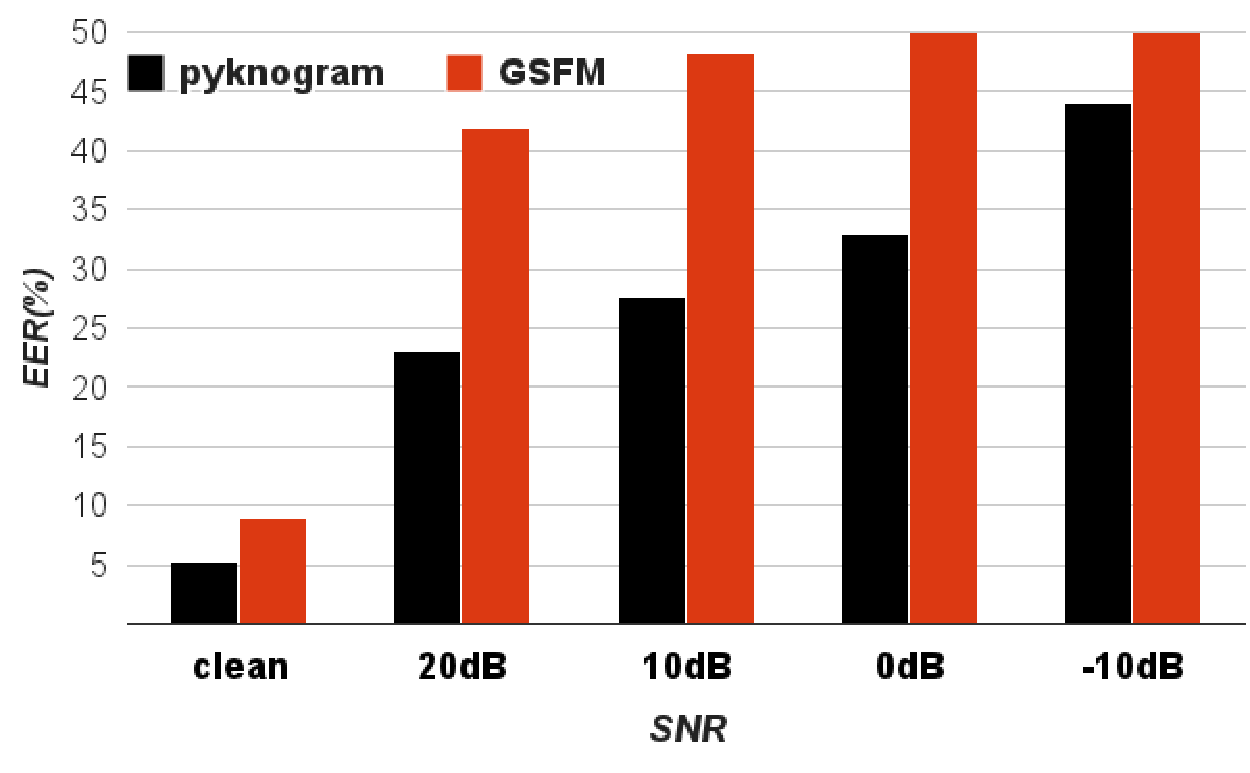
\includegraphics[height = 2.8in, width=0.8\textwidth]{figures/pykno_vs_GSFM}
	\caption{\it A comparison of overlap detection equal error rates (EER) for pyknogram (proposed) and GSFM-based systems for different amounts of added noise. It is clear that GSFM is vulnerable even to the slightest amount of noise (high SNR).}
	\vspace{-1mm}
	\label{fig:ovl_detect_eer_noise}
\end{figure}


Performances from other overlap detection algorithms were not included here, since to the best of our knowledge none of the existing algorithms claim robustness in noisy conditions. 

\newpage
\section{Summary}
\label{sec:ch2_summary}
The focus of this chapter was on overlapped speech, which refers to segments where both speakers (primary and interferer) are active. 
Independent cross-talk data (as defined in Chapter~\ref{chap:intro}) were used in order to isolate overlap from other forms of interference, such as noise.
Two overlap detection methods were proposed: Pyknogram, and GSFM. 
Pyknograms are useful for overlap detection, since they enhance speech harmonics regardless of the number of speakers in a signal. 
The noticeable difference between single-speaker and overlap harmonics allows Pyknograms to be an asset to overlap detection. 
The second method, GSFM, magnifies dispersive trends in speech sub-bands in the presence of overlap using multi-tone frequency modulation analysis. 
The two proposed methods are compared in real environmental noise and it is shown that despite outperforming Pyknograms in clean conditions, GSFM is highly affected by adding noise in overlap detection experiments. 
Therefore, Pyknograms provide more robust overlap detection performance. 

